\documentclass[aps,prd,reprint,floatfix,nofootinbib,longbibliography]{revtex4-2}
\usepackage[T1]{fontenc}
\usepackage{amsmath,amssymb,bm,graphicx,booktabs}
\usepackage[colorlinks=true,linkcolor=blue,citecolor=blue,urlcolor=blue]{hyperref}
\graphicspath{{figures/}}
\newcommand{\scri}{\mathscr I^+}
\newcommand{\Iplus}{\mathcal I^+}
\newcommand{\Ar}{\mathcal A}
\newcommand{\Kh}{\widehat K}
\newcommand{\Th}{\Theta}
\newcommand{\HH}{\mathcal H}
\newcommand{\MM}{\mathcal M_r}
\newcommand{\dd}{\mathrm d}
\newcommand{\normr}[1]{\left\|#1\right\|_r}
\newcommand{\code}[1]{\texttt{\detokenize{#1}}}
\newcommand{\tcell}[1]{{\raggedright #1\par}}
\begin{document}
\title{Elliptic-shift hyperboloidal evolution in spherical symmetry:
formulation, numerical verification, and strong-field limitations}
\date{Working manuscript; evidence snapshot of 27 October 2026}
\begin{abstract}
We investigate a spherical free-evolution formulation of the conformally compactified Einstein equations in which a live hyperboloidal lapse is coupled to an elliptic shift derived from the conformal metric connection. The shift condition does not constrain the independently evolved Z4 connection variable. We describe nonlinear spherical equations, actual-null-infinity boundary treatment, positive field variables, a separate asymptotically flat puncture chart, and coupled massless-scalar evolution. Independent tensor comparisons, stage-by-stage shift solves, and restart tests support implementation consistency. A finite-amplitude Minkowski lapse pulse exhibits observed orders of $5.00$ in the bulk and $4.20$ near null infinity over $0\leq t\leq1$, although the finest constraint measurements encounter an arithmetic floor. A coupled subcritical scalar experiment gives a final mass--flux discrepancy of $8.19\times10^{-9}$ on the finest tested grid. Historical wormhole trials develop unresolved steep gauge fronts, and causal retained-domain evolutions have insufficient constraint convergence despite reaching $t=10$. A subsequent spherical conformal telegrapher lapse adds a relaxation flux and tracks the coupled gauge characteristics at every Runge--Kutta stage. We report a full-domain, three-resolution follow-up through $t=10$, with bulk field order $5.89$ and finest peak accepted Hamiltonian RMS $1.53\times10^{-8}$. The fixed candidate passes the stated spatial checks, while retaining a narrow nonmonotone inner lapse structure and strong finite-grid characteristic compression. A single-grid continuation targeting $t=500$ stops at $t=43.8365$ at a gauge/positivity guard. The exterior constraint budget remains nearly steady through the last saved time $t=43.8$, with relative apparent-horizon mass error $1.18\times10^{-7}$. Interior errors are recorded separately and excluded from this budget; the target duration was not reached. Offline replay identifies fourth-stage lapse underflow near the puncture. A configurable physical-lapse floor permits a short control to pass that event. A fresh floored trial then stops at $t=84.7983$ on the coupled-speed timestep guard, driven by a large inner shift; its final saved relative horizon-mass error is $2.10\times10^{-7}$. The floor prevents the diagnosed underflow but does not establish long-time stability. A separate candidate combines total-lapse Runge--Kutta stages, positive-radius inner stencils, and a lapse-dependent attenuation of the telegrapher coupling. Its interim $N=1025$ trajectory passes the declared exterior accuracy budget through $t=90$, beyond the earlier stopping time, while retaining small inner lapse ripples. The $t=500$ duration assessment remains pending. Independent quadrature, dissipation-amplitude, and adjacent relaxation-parameter controls remain unrun; robust nonlinear stability is therefore not established. An already-trumpet control with a separate analytic lapse source reaches $t=100$ with small invariant errors, but does not establish wormhole-to-trumpet evolution in the main gauge. We retain negative results and distinguish algebraic verification, short-time convergence, and unresolved nonlinear stability. No successful coupled collapse, quasinormal-mode extraction, or late-time-tail result is claimed.
\end{abstract}
\maketitle
\section{Introduction}
Hyperboloidal slices place future null infinity at a finite coordinate location while retaining a spacelike initial-value surface. They therefore offer direct access to outgoing radiation, but conformal compactification introduces formally singular coefficients into free-evolution equations. Spherical calculations have established that gauge choices and constraint damping are central to obtaining regular numerical evolutions\cite{VHH2015,VH2014,VH2018}. Black-hole trumpet constructions, dynamical conformal diagrams, and alternative reference metrics provide complementary tests of the same asymptotic difficulty\cite{VV2023,VV2024,VVValente2024}.

The present experiment replaces a hyperbolic shift driver by a condition on the \emph{metric-derived} reference connection. The distinction matters: freezing a connection computed from the metric need not suppress an independently evolved connection constraint. Our aim is to retain free Z4c evolution while controlling conformal metric shape through an elliptic gauge solve. The supplied linearized closure notes motivate this construction, but concern a compatible perturbative phase around hyperboloidal Minkowski spacetime. They do not establish nonlinear black-hole or Einstein--scalar stability.

This paper reports the evidence presently available, including unsuccessful variants. Its principal new strong-field result is a full-domain, three-grid telegrapher lapse study through $t=10$, which passes the declared spatial checks while retaining a narrow inner lapse feature and strong characteristic compression. This result complements implementation checks, weak-field convergence, and coupled subcritical mass--flux tests; it does not establish long-time nonlinear stability. The failed pre-telegrapher front is preserved in Appendix~\ref{app:pre-telegrapher}. The different experiments use explicitly labeled gauge and numerical variants; they do not constitute a single universally successful parameter choice. We distinguish an exact identity, agreement between implementations, convergence of a numerical experiment, and successful completion of a physical scenario throughout.

\section{Nonlinear spherical formulation}
\label{sec:formulation}
\subsection{Fields and conventions}
We set $G=c=1$ and use the compactification length as the unit of length and time. The fixed conformal factor and Minkowski reference are
\begin{equation}
 \begin{gathered}
 \Omega=(1-r^2)/2,\qquad A=(1+r^2)/2,\\
 \beta_\star=-r,\qquad K_\star=-3.
 \end{gathered}
\label{eq:reference}
\end{equation}
The outer boundary is the actual grid point $r=1$ at $\Iplus$. The physical metric is $\widetilde g_{ab}=\Omega^{-2}\bar g_{ab}$, with conformal lapse $\alpha$, radial shift $\beta$, and spatial line element
\begin{equation}
 \dd\widetilde\ell^2=\frac{1}{\Omega^2\chi}
 \left[g\,\dd r^2+r^2g^{-1/2}\dd\omega^2\right].
\label{eq:metric}
\end{equation}
The physical lapse is $\widetilde\alpha=\alpha/\Omega$. The freely evolved geometric fields are
\begin{equation}
 (\chi,g,\Ar,\Kh,\Th,\Lambda^r,\alpha),\qquad
 \Kh=K-2\Th,
\end{equation}
where $K$ and $\Th$ have physical normalization and $\Ar=A_{rr}$ is the conformal radial trace-free curvature variable, normalized so that $K^r{}_r-K/3=\Omega\Ar/g$. The angular metric and curvature components follow from the algebraic determinant and trace conditions. These algebraic reductions do not solve the Hamiltonian or momentum constraints.

The spherical restriction retains angular tensor derivatives. For example, the transverse Hessian of a radial scalar is $f_r/r$; vector and tensor derivatives contain additional angular terms. A native tensor implementation constructs these derivatives explicitly and supplies an independent comparison for the canceled radial implementation. Most evolution results use initially isotropic conformal data, $g=1$, for which the metric-freezing gauge preserves $g=1$. Appendix~\ref{app:equations} gives the corresponding nonlinear vacuum equations and constraints. The remaining curvature, trace, and Z4 variables stay independent.

\subsection{Metric-derived elliptic shift}
Let $V^r$ denote the contracted connection difference computed from the conformal metric and the flat spherical reference connection. Direct contraction gives
\begin{equation}
 V^r=\frac{g_r}{g^2}+\frac{2}{r}\left(\sqrt g-\frac1g\right),
 \qquad Z_r=\frac g2(\Lambda^r-V^r).
\label{eq:V}
\end{equation}
In particular, $V^r$ and $\Lambda^r$ are different quantities off the constraint surface. Write the radial metric rate as
\begin{equation}
 Q\equiv\partial_tg=\beta g_r+\frac{4g}{3}
 \left(\beta_r-\frac\beta r\right)-2\alpha\Ar.
\end{equation}
Differentiating Eq.~\eqref{eq:V} yields
\begin{equation}
 \partial_tV^r=\frac{1}{g^2}(Q_r+P_g Q),\qquad
 P_g=-\frac{2g_r}{g}+\frac{g^{3/2}+2}{r}.
\end{equation}
The gauge $\partial_tV^r=-\eta_D V^r$, with $\eta_D\geq0$, is therefore a second-order radial equation for $\beta$. With $C_g=4g/3$ and $D_g=g_r-4g/(3r)$, it reads
\begin{align}
 C_g\beta_{rr}+(C_{g,r}+D_g+P_gC_g)\beta_r
 &+(D_{g,r}+P_gD_g)\beta \nonumber\\
 =2(\alpha\Ar)_r+2P_g\alpha\Ar&-\eta_Dg^2V^r.
\label{eq:elliptic}
\end{align}
Its principal coefficient is positive for $g>0$.

For $g=1$ and metric freezing, the homogeneous metric-rate equation is $Q_r+3Q/r=0$. Center regularity excludes $Q\propto r^{-3}$, leaving $Q=0$. The analogous bounded-shape condition excludes this mode at the asymptotically flat inner end. Defining $W=(\beta+r)/r$, one obtains
\begin{align}
 W_r&=\frac{3\alpha\Ar}{2r},\label{eq:W}\\
 W(1)&=-\frac{c+(2u+u^2)\chi}{1+\alpha\sqrt\chi}\bigg|_{r=1},\nonumber
\end{align}
where $c=\chi-1$ and $u=\alpha-A$.
The boundary value is an algebraically stable form of the null-normal shift condition. It fixes the remaining homogeneous shift mode. Thus $\beta$ is determined without using $\Lambda^r$, $\HH$, or $\MM$. At a later finite cutoff, $Q=0$ is retained as an explicit inherited elliptic gauge condition; the regular-center uniqueness argument is not reapplied to that truncated domain.

\subsection{Live lapse and disclosed source variants}
With $v=\beta+r$ and $p=\Kh$, the baseline lapse equation is
\begin{align}
 \partial_t\alpha={}&\beta u_r+rv+\frac{S_\alpha}{\Omega},\nonumber\\
 S_\alpha={}&-F(p+3)+r(Av-ru+uv)-\mathcal D,\label{eq:lapse}\\
 F={}&\alpha^2+4\nu\Omega^2\alpha.\nonumber
\end{align}
The term proportional to $\alpha$ gives logarithmic-slicing-like behavior in the interior, whereas $F\to\alpha^2$ at scri. This is not exact physical $1+\log$ slicing at every interior point. The pulse experiments use $\nu=1$ and symmetric restoring,
\begin{equation}
 \mathcal D_{\rm sym}=\xi(\alpha+A)(\alpha-A),\qquad\xi=1.
\end{equation}
This restoring term is an explicit gauge modification relative to the original un-restored reference prescription.

The same untapered symmetric source obstructs a regular stationary collapsed lapse at a puncture. If $\alpha\sim r^\gamma$, $\gamma>0$, $\beta=O(r)$, and $\Kh$ stays finite, the other lapse terms vanish at $r=0$, but
\begin{equation}
 \partial_t\alpha(0)=\frac{\xi}{2}.
\label{eq:obstruction}
\end{equation}
This conditional statement concerns that source choice, not free Z4c or elliptic shifts in general. A multiplicative control,
\begin{equation}
 \mathcal D_{\rm mult}=2\xi\alpha(\alpha-A),
\end{equation}
removes the constant and differs from the symmetric lapse numerator by $-\xi u^2$. It preserves the linearization about Minkowski, but does not by itself provide stable black-hole evolution.

The later wormhole tests also use
\begin{align}
 \xi_{\rm eff}(r)&=\xi+(3\nu-\xi)(2\Omega)^4,\nonumber\\
 \Delta S_\alpha&=(2\Omega)^4r^2\frac{\alpha-A}{A},
\label{eq:physical-log}
\end{align}
with multiplicative restoring. These changes preserve the Minkowski equilibrium and the leading scri limits, but \emph{change the interior linearized gauge}. We refer to this as the modified logarithmic source. The main black-hole tests retain the Minkowski lapse reference. A distinct already-trumpet control adds an analytic CMC lapse source; it is identified separately in Sec.~\ref{sec:cmc}.

\subsection{Off-constraint terms}
The candidate uses $\kappa_1=4$, $\kappa_2=-0.99$. The scalar-$\Th$ equation differs from the repository control by
\begin{equation}
 \Delta(\partial_t\Th)=\frac{3\alpha w\Th}{\Omega},\qquad
 w=\bar n(\Omega)=\frac{\beta r}{\alpha}.
\label{eq:theta-change}
\end{equation}
This removes a repository $-3\alpha w\Th/\Omega$ term and implements the tested Appendix-C-style choice\cite{VHH2015}. The change vanishes on the constraint surface, but changes the off-constraint system. Agreement with the native implementation alone does not constitute a complete independent audit of every published Appendix C term.

A separate reference-lapse damping control replaces products $\alpha\kappa_1$ by $A\kappa_1$. The implementation evaluates those products directly, avoiding division by a collapsed lapse. This changes damping away from the constraint surface. We do not combine results from this control with constant-damping experiments as if they used identical equations.

\begin{figure*}[tp]
 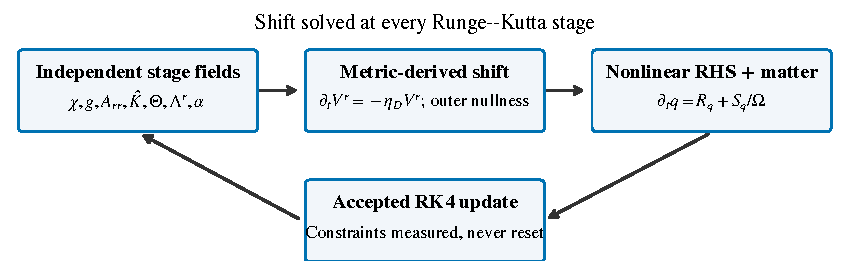
\includegraphics[width=\textwidth]{scheme}
 \caption{Stage structure of the method. The elliptic equation controls the metric connection, while $\Lambda^r$, $\Th$, curvature, and the trace remain evolved fields. The diagram describes the algorithm, not a stability theorem. Scalar sources and radiation flux, when present, are evaluated at the same RK stages.}
 \label{fig:scheme}
\end{figure*}

\section{Regularization and numerical implementation}
\label{sec:numerics}
\subsection{Actual scri and the boundary clock}
Each geometric equation is assembled as $\partial_tq=R_q+S_q/\Omega$, combining its entire numerator before division. For a regular compatible solution, $S_q(1)=0$ and
\begin{equation}
 \partial_tq(1)=R_q(1)-\partial_rS_q(1),
\label{eq:limit}
\end{equation}
because $\Omega_r(1)=-1$. Both differentiation of the combined numerator and analytic product-rule evaluation have been tested. No floor is applied to $\Omega$.

The lapse clock and null boundary condition are
\begin{equation}
 \alpha(1)=1,\quad \partial_t\alpha(1)=0,\quad
 \beta(1)=-\alpha(1)\sqrt{\chi(1)/g(1)}.
\end{equation}
Only the lapse rate is set by the clock. The other endpoint fields evolve. Naive use of Eq.~\eqref{eq:limit} on unrestricted nodal data is unstable in the tested system. The candidate therefore adds weak endpoint terms
\begin{equation}
 (\partial_tq)_1\longmapsto(\partial_tq)_1+
 \frac{\sigma S_q(1)}{h}-\frac{\tau\mathcal C_q(1)}{h},
 \qquad (\sigma,\tau)=(4,8).
\label{eq:penalty}
\end{equation}
For the $g=1$ field order used above,
\begin{equation}
 \mathcal C=(\chi-1,0,\Ar+2\chi_r/3,p+3,\Th,\Lambda^r,0).
\end{equation}
These traces vanish in the intended regular boundary phase. The terms are additional numerical boundary penalties, not a projection of bulk constraints and not a proven nonlinear energy closure. Their residues and convergence are measured explicitly.

The clock alone does not establish Bondi-time affinity. In the unit-sphere conformal frame $g_B=\chi\bar g$, the scri generator has nonaffinity
\begin{equation}
 \kappa_B=\frac{\chi_t}{2\alpha\chi}
 -\frac{\chi_r}{2\sqrt\chi}
 -\frac{\sqrt\chi\,\alpha_r}{\alpha}-\frac{\beta_r}{\alpha}.
\label{eq:affinity}
\end{equation}
The actual numerical endpoint rate enters this expression. With $\alpha(1)=1$, a normalized affine parameter satisfies $\dd\lambda/\dd t=\exp(\int_0^t\kappa_B\dd s)$. We monitor $\kappa_B$ independently of clock and nullness errors.

\subsection{Spatial operators, stage solves, and arithmetic}
Regular-center runs normally use the half-cell grid $r_i=(i+1/2)/(N-1/2)$, $i=0,\ldots,N-1$, with actual scri. Seven-point polynomial finite differences are sixth order in the centered interior; one-sided closures have their own consistency orders. Reflected tensor parity supplies the center. $\Ar=O(r^2)$ and $\Lambda^r=O(r)$ are stronger requirements than even and odd parity alone. The usual time step is $\Delta t=C_{\rm CFL}h$ with $C_{\rm CFL}=0.05$, and integration uses classical RK4.

Two shift discretizations are available. Local interpolatory interval quadrature integrates Eq.~\eqref{eq:W} in $O(N)$ work. Summing tails from scri avoids subtraction of two large prefix integrals. Alternatively, a banded discrete derivative equation for $W$ is factored once and solved at every RK stage. A one-point right-biased derivative in this \emph{shift solve} removes an unstable finite-grid mode found with the centered matrix. This bias is distinct from optional biased transport in the evolution equations. The banded solve costs $O(Ns)$ per stage after $O(Ns^2)$ setup, where $s$ is the fixed stencil width. Residual corrections with zero, two, and four passes provide an arithmetic control. On this host, \code{long double} has the same 53-bit significand as binary64; the corrections are not an extended-precision evolution.

The small banded-system residual and the residual obtained by independently differentiating sampled $\beta$ measure different errors. The latter includes interpolation and discrete product-rule errors. Neither is silently substituted for the other. Changing quadrature degree also changes a spatial discretization and is assessed separately from correcting a fixed linear system.

The regular-center Kreiss--Oliger filter uses sixth differences with a fixed taper that vanishes outside $r<0.4$. Applying it to $\Ar/r^2$ and $\Lambda^r/r$ respects their center scaling. Its strength is usually $\epsilon=0.5$; its $h^5$ contribution can limit the observed spatial order. At a puncture the filter instead has the form $-\epsilon B^TWB/(64h)$, where $B$ is a third forward difference and $W\geq0$. It uses no center parity. At a finite cutoff, multiplying the weight by $d^6/(L^6+d^6)$, with $d$ the stencil-midpoint distance from the cutoff, improves the first-active-row consistency. A negative filter energy contribution alone does not imply stability of the coupled equations.

Two arithmetic repairs are useful. Difference-form differentiation, $\sum_jD_{ij}(q_j-q_i)$, removes floating-point derivative row sums acting on constants. Compensated accumulation of accepted RK increments reduces loss in repeated additions. The correction is explicit checkpoint state. Stage evaluations remain binary64; neither repair produces a higher-precision solution. An integer-step clock records $t=t_0+(n-n_0)\Delta t$ and prevents cumulative timestamp drift. Older frozen trajectories retain their original clock limitations.

\subsection{Positive variables and inner ends}
For a regular center we optionally evolve
\begin{equation}
 \chi=e^U,\qquad \alpha=Ae^V,
\end{equation}
using the exact chain rules $U_t=\chi_t/\chi$ and $V_t=\alpha_t/\alpha$. Deviations are evaluated with \code{expm1} and \code{log1p}, and positive totals are passed directly to the geometric and matter kernels. This avoids recovering a small positive total by adding it to an order-one negative deviation. The historical experiments, including the completed three-grid telegrapher study and the original long-duration attempt, terminate on overflow, underflow, or invalid totals without a positivity floor. The separate configurable-floor extension is described in Sec.~\ref{sec:lapse-floor}. Dissipation acts on stored variables, so changing variables also changes the finite-grid filter.

The wormhole's other end is not a regular center. Its asymptotic phase is
\begin{align}
 \chi&=r^4X,\quad \alpha=r^2a_2,\quad\Lambda^r=\ell_0,\nonumber\\
 (\Ar,p,\Th)&=r^2(b_2,k_2,\theta_2).
\end{align}
Odd powers in the coefficient expansions are allowed. A reference-scaled positive chart evolves an actual $r=0$ coefficient node. For multiplicative restoring, before Eq.~\eqref{eq:physical-log}, the leading lapse coefficient obeys
\begin{equation}
 \dot a_2=(2b_1-6\nu+2\xi)a_2+2,
 \qquad \beta=b_1r+\cdots.
\end{equation}
The modified source in Eq.~\eqref{eq:physical-log} gives $\dot a_2=2b_1a_2$ for the linear slicing family. The other leading free coefficients have rates $2b_1$ times the coefficient for constant damping. Independent tensor limits check these equations. The coefficient node represents spatial infinity; positivity of the physical metric is tested at $r>0$.

For finite retained domains, physical curvature variables can be better conditioned than the asymptotically flat scalings. We tested
\begin{equation}
 \chi=p_\chi(r)e^U,\qquad p_\chi=\frac{r^2}{A^2},\qquad
 \alpha=Ae^V,
\label{eq:trumpet-chart}
\end{equation}
while retaining physical $\Ar,p,\Th,\Lambda^r$. A compact alternative equals this profile below $r=0.1$ and becomes exactly one beyond $r=0.3$. Both are coordinate-only variable profiles, independent of black-hole mass and of the lapse gauge source. Writing $X=\chi/r^2$ and $\ell=(\log X)_r$ cancels the leading inner powers analytically. In particular,
\begin{equation}
 \MM=\Omega(\Ar_r-\tfrac32\Ar\ell)-\tfrac23K_r+2r\Ar
\end{equation}
in vacuum. No constraint is used to obtain this identity.

A domain transfer is allowed only from an exact saved subset of a completed full-domain trajectory. It records the original profile, equation parameters, time lattice, and source hashes. Every subsequent stage requires the maximum physical and gauge speeds at the left boundary,
\begin{equation}
 -\beta+\alpha\sqrt\chi,\qquad -\beta+\sqrt{F\chi},
\end{equation}
to remain negative. Transfer to Eq.~\eqref{eq:trumpet-chart} preserves curvature and Z4 fields bitwise and measures the logarithmic reconstruction error. A retained-domain result cannot certify the discarded region or replace assessment of the entire preceding trajectory.

\subsection{Coupled massless scalar}
Let $R=r/(\Omega\sqrt\chi)$ be the areal radius for $g=1$. The stored scalar fields are
\begin{equation}
 f=\frac{R\phi}{r}=\frac{\phi}{\Omega\sqrt\chi},\qquad
 P=\frac{\bar n(R\phi)}{r}.
\end{equation}
With $k=K/3-\Omega\Ar/2$, the conformal normal derivative is
\begin{equation}
 \Pi\equiv\bar n(\phi)=\sqrt\chi(\Omega P+kf).
\end{equation}
The physical normal derivative is $\Omega\Pi$. Matter contributions are included in both the evolution and constraint diagnostics. The radius-weighted wave equation retains the angular Ricci contribution produced by the free Z4c geometry; setting it to its on-constraint value would change the off-constraint scalar equation. Explicit formulas are collected in Appendix~\ref{app:matter}.

Scalar initial data solve the Hamiltonian equation for $\psi=1+\Omega^3w$ and $\chi=\psi^{-4}$, with $K=-3$, $\Ar=\Th=\Lambda^r=0$, and $\Pi=0$. The regular outer condition is $w_r(1)=-3w(1)$ and the initial Bondi mass is $8w(1)$. High-precision residual evaluation was introduced when a requested Newton tolerance met the binary64 residual floor. This is an initialization solve, never an evolution projection. Radiation energy is accumulated with RK-stage fluxes $4\pi(\partial_tf|_{\Iplus})^2$; coordinate-time and Bondi-time interpretations are distinguished using Eq.~\eqref{eq:affinity}.

\section{Verification and assessment protocol}
\label{sec:protocol}
The historical implementation snapshot used for the results in Sec.~\ref{sec:results} contains 50 passing test groups; the later telegrapher checks are reported separately in Sec.~\ref{sec:telegraph}. It includes tensor and radial comparisons, manufactured shift solutions, selected independent ADM and scalar identities, scri and inner-end limits, and bitwise restart checks. The 128-case physical-trumpet-chart audit covers vacuum and scalar rates, transport, damping, endpoints, and short steps. Its maximum native-tensor, compiled/Python, and short-step discrepancies are $3.91\times10^{-14}$, $2.84\times10^{-14}$, and $8.89\times10^{-16}$, respectively. These are implementation checks rather than physical evolution results.

Our physical-field comparison uses an $r^2$-weighted nodal RMS,
\begin{equation}
 \normr{e}=\left[\frac{\sum_{i\in\mathcal R}r_i^2
 \sum_a e_{ia}^2}{\sum_{i\in\mathcal R}r_i^2}\right]^{1/2}.
\end{equation}
The compared geometric fields are the physical deviations and free curvature/Z4 fields, excluding the unused shift placeholder. Bulk and endpoint regions are $r<0.8$ and $r>0.9$. These are diagnostic norms, not invariant energy norms. Nested grids use exact restriction; half-cell comparisons use degree-eight spatial interpolation. No temporal interpolation or relabeling of old frames is used. Orders are fitted with the actual grid spacings, rather than assuming an exact factor of two for half-cell grids.

Predeclared preliminary requirements include strict metric/lapse positivity, clock error below $10^{-13}$, nullness error below $10^{-12}$, geometric and lapse pole residues below $10^{-7}$, bulk gauge-pulse constraint order at least $3.5$, endpoint field order at least $3$, and independently estimated time/elliptic errors below $10\%$ of the spatial error. These criteria are necessary checks, not substitutes for physical invariants, long durations, or independent parameter controls.

Every RK stage is checked for safety and compatibility. Accuracy of constraints is also monitored at accepted states: an intermediate RK trial state is not a fourth-order approximation to the exact intermediate solution. We do not infer accepted-step coverage for older records that contain only sampled reports. Cumulative maxima include earlier transients and the last accepted state; a quiet endpoint cannot erase a previous failure.

\section{Numerical results}
\label{sec:results}
Table~\ref{tab:experiments} identifies the historical experiment families. All times are in compactification units, not automatically in units of the black-hole mass. The historical runs in this section were already available for the original manuscript. Section~\ref{sec:telegraph} reports the subsequently authorized telegrapher investigation separately.

\begin{table*}[tp]
\caption{Principal historical evidence families. ``Completed'' means the integrator reached its target, not that the scientific acceptance criteria passed. All listed coupled evolutions use actual scri. Q denotes quadrature shift integration and B denotes the right-biased discrete shift equation. The independent scalar solver is a separate fixed-background control.}
\label{tab:experiments}
\begin{ruledtabular}
\begin{tabular}{p{2.9cm}p{5.2cm}p{3.0cm}p{4.8cm}}
\tcell{Experiment} & \tcell{Gauge / numerical choice} & \tcell{Resolution and duration} & \tcell{Supported interpretation}\\
\hline
\tcell{Finite lapse pulse} & \tcell{$\nu=1$, symmetric restoring; positive variables; B; compensated increments} & \tcell{$2048,4096,8192$; $t=1$} & \tcell{High-order field convergence; finest constraint floor}\\
\tcell{Small lapse pulse} & \tcell{$\nu=1$, symmetric restoring; older primitive-variable Q implementation} & \tcell{$256,512$; $t=10^4$} & \tcell{Long survival; finest continuation paused near $8250$}\\
\tcell{Already-trumpet CMC} & \tcell{Analytic CMC lapse source; symmetric restoring; reference-lapse damping; Q} & \tcell{$256,512,1024$; $t=100$} & \tcell{Small mass drift; separate gauge control}\\
\tcell{Full wormhole prefix} & \tcell{Modified logarithmic source; $\nu=0.25$; AF coefficient chart; Q} & \tcell{$2049,4097,8193$; $t=3.2$} & \tcell{Resolved early physical fields; finest $\HH$ floor}\\
\tcell{Retained wormhole domain} & \tcell{Same gauge; global trumpet metric profile; physical curvature; Q} & \tcell{$1009,2017,4033$; $3.2\leq t\leq10$} & \tcell{All reach target; transient constraint order inadequate}\\
\tcell{Coupled dispersal} & \tcell{$A_\phi=0.058$; $\nu=1$; symmetric restoring; Q} & \tcell{$512,1024,2048$; $t=6$} & \tcell{Convergent mass--flux check; finest component gates pass}\\
\tcell{Collapse trial} & \tcell{$A_\phi=0.07$; $\nu=0.25$; modified source; positive upwind variables; Q} & \tcell{$512,1024,2048$; $t=3$} & \tcell{Large, nonconvergent constraints; failed experiment}
\end{tabular}
\end{ruledtabular}
\end{table*}

\subsection{Minkowski equilibrium and finite lapse pulses}
The reference fields in Eq.~\eqref{eq:reference}, with $\chi=g=1$ and $\Ar=\Th=\Lambda^r=0$, provide an unsubtracted equilibrium check. Analytic cancellation and constant-nullspace differentiation are particularly important here: otherwise derivatives of an order-one background can seed resolution-dependent curvature noise. Successful equilibrium tests do not certify a finite perturbation or the strong-field regime.

The finite-amplitude study starts with the lapse perturbation
\begin{equation}
 \begin{gathered}
 u(0,r)=a_\alpha\exp\left[-\frac{(r^2-r_c^2)^2}{4s^4}\right],
 \\
 (a_\alpha,r_c,s)=(0.1,0.25,0.1),
 \end{gathered}
\end{equation}
and unperturbed geometric data. This is the published-form pulse used as a physical test, not a claim of identical published gauge evolution. On $N=2048,4096,8192$ at fixed CFL, the peak-in-time physical-field difference has observed order $5.0004$ in the bulk and $4.2005$ near scri. Time-RMS orders are $4.9975$ and $4.2089$. Figure~\ref{fig:gauge} shows the underlying differences, including the pulse's passage through the outer region. The approximately fifth-order bulk behavior is consistent with the filter contribution; it should not be described as a uniform sixth-order evolution.

\begin{figure*}[tp]
 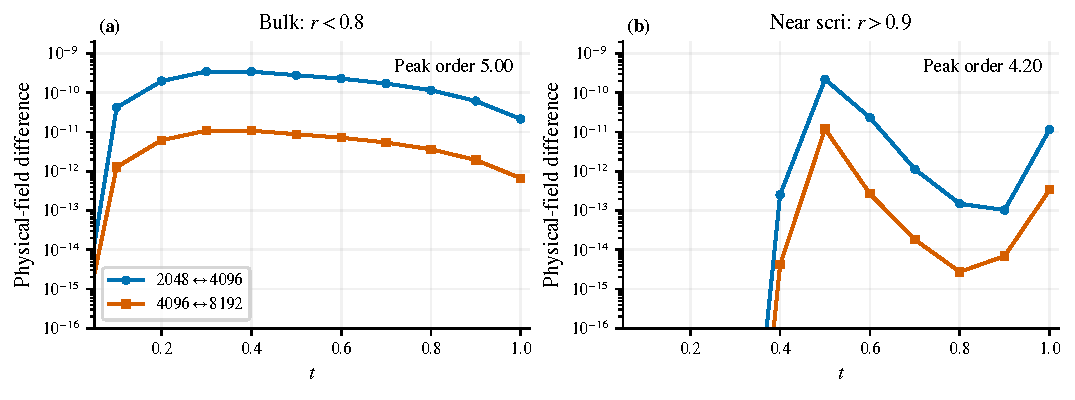
\includegraphics[width=\textwidth]{gauge_convergence}
 \caption{Finite-amplitude lapse pulse with local derivative subtraction and compensated accepted updates. Curves are differences between consecutive resolutions in physical variables at exact common saved times. The peak-difference orders are $5.00$ in the bulk and $4.20$ near scri. Values below the plotted range at early times reflect the initially negligible outer signal, not measured asymptotic convergence. This experiment ends at $t=1$.}
 \label{fig:gauge}
\end{figure*}

The constraint results are more restrictive. Figure~\ref{fig:arithmetic} compares local derivative subtraction with and without compensated accepted increments. At $N=8192$, the peak accepted-state Hamiltonian RMS decreases from $9.99\times10^{-10}$ to $7.88\times10^{-11}$, and the momentum RMS decreases from $7.63\times10^{-10}$ to $5.68\times10^{-11}$. Compensation substantially reduces the arithmetic contamination, but the finest Hamiltonian error still increases relative to $N=4096$. A field-convergence plot alone would miss this limitation.

\begin{figure*}[tp]
 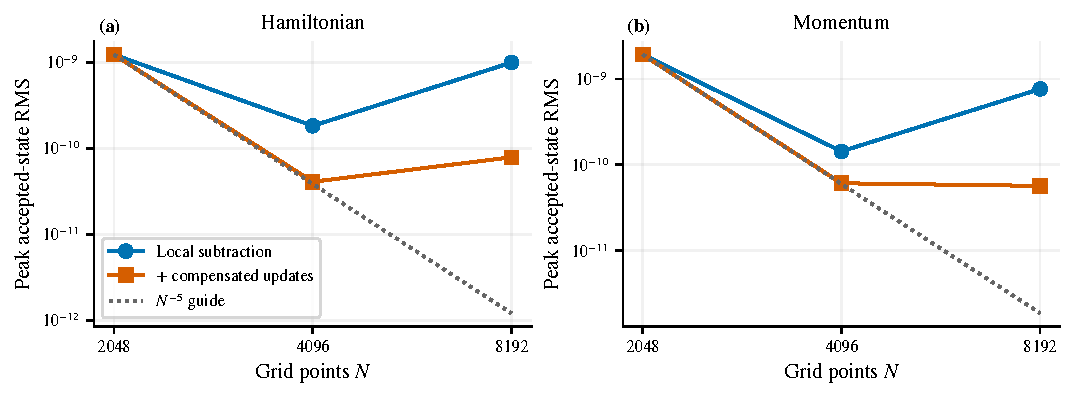
\includegraphics[width=\textwidth]{arithmetic_floor}
 \caption{Peak constraints over all accepted states of the finite pulse on $0\leq t\leq1$. The dotted lines are fifth-order reference slopes, not fits. Compensated updates reduce the finest errors, but do not remove the constraint floor. Intermediate RK trial-state constraints are not substituted for accepted-state accuracy.}
 \label{fig:arithmetic}
\end{figure*}

Independent $N=4096$ controls support separation of time and shift-solve errors from the measured field differences. Halving the timestep changes the final bulk and endpoint fields by $8.07\times10^{-15}$ and $2.44\times10^{-16}$, respectively. These are about $1.17\%$ and $0.070\%$ of the corresponding middle-grid Richardson estimates. Changing the number of banded residual corrections from two to zero or four gives bulk fractions of $1.30\%$ and $1.27\%$, and endpoint fractions below $0.065\%$. One timestep halving does not establish RK4 order; a separate earlier, coarser control resolved RK4. The compensated finest-grid study remains a short-time component result.

The small-amplitude $a_\alpha=10^{-3}$ runs are a different, older implementation family. Two resolutions reached $t=10^4$. The $N=1024$ continuation is paused near $t=8250$, and its accumulated timestamps exhibit the older clock drift. These runs provide long-survival evidence but do not complete a three-resolution long-duration assessment of the later $a_\alpha=0.1$ scheme. Compatible independent constraint perturbations and resolution-scaled noise have also been exercised. Smooth supported constraint perturbations at $N=128,256,512$ reach $t=10$ and decay. The original fixed-amplitude nodal-noise sequence reaches $t=6$, but its finest-grid $\Th$ amplification, $129.5$, exceeds the declared per-component limit of $100$. This remains a failed test. High-frequency metric noise enters $\HH$ through second derivatives, so a fixed nodal amplitude does not bound the mixed-derivative perturbation size uniformly under refinement.

A separately specified, derivative-balanced dataset scales the $\chi$ perturbation as $h^2$ and the independent curvature, $\Kh$, $\Th$, and connection perturbations as $h$. With amplitude parameter $10^{-5}$ and seed $7419$, all four grids $N=128,256,512,1024$ reach $t=6$ and pass the boundary, positivity, component-amplification, and final-decay gates. On the finest grid the peak amplification factors for $(\HH,\MM,\Th,Z_r)$ are approximately $(1.46,1.00,1.15,7.20)$, and the final-to-initial ratios are below $3.1\times10^{-7}$. This is a distinct perturbation experiment, not a retrospective pass for unscaled noise or a spatial-convergence study of fixed continuum data. A comprehensive long-duration robust-stability assessment is still absent.

\subsection{Endpoint and discrete-shift failures}
\label{sec:endpoint-failures}
The naive l'Hopital endpoint treatment has a readily identifiable discrete failure. The scalar model $T_t=-cT/\Omega$, extended at scri by $T_t=cD_rT$, contains a positive diagonal endpoint contribution. In the recorded $N=24$ comparison, the full endpoint-localized mode grows at approximately $232.44$, close to the model value $232.60$. This does not contradict a continuum statement restricted to compatible weighted data. It demonstrates that the unrestricted nodal phase is larger than that continuum phase. Extrapolating the combined quotient reduced, but did not remove, the observed instability.

A second failure arises even when the discrete elliptic system is solved accurately. The centered shift-ODE variant fails the finite pulse near $t=0.7073$, $0.2970$, and $0.1055$ at $N=512,1024,2048$. Timestep halving does not repair the middle-grid failure. Its coupled finite-grid Jacobian has growing outer-localized modes; the dominant real part reaches $44.66$ at $N=512$. The right-biased variant has a dominant real part near $-0.706$ on the tested grids [Fig.~\ref{fig:endpoint}(a)]. These spectra diagnose the tested discrete systems; they are not continuum or nonlinear stability proofs.

Finally, a successful final-time convergence check can be misleading. The original right-biased $512/1024/2048$ study gives endpoint order $4.82$ at $t=1$, but only about $1.28$ at $t=0.5$ [Fig.~\ref{fig:endpoint}(b)]. The fixed-grid timestep difference at that transient is $5.76\times10^{-14}$, far below the spatial discrepancy. Refinement and arithmetic controls, rather than a new time integrator, were therefore the relevant next tests. The finer result in Fig.~\ref{fig:gauge} improves this behavior, without retroactively making the coarse experiment acceptable.

\begin{figure*}[tp]
 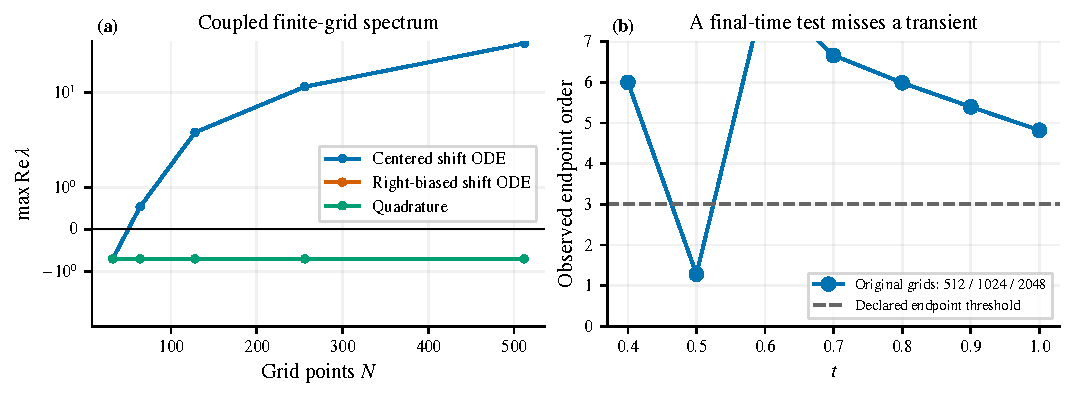
\includegraphics[width=\textwidth]{endpoint_failures}
 \caption{Two distinct endpoint-related failures. (a) Dominant real eigenvalue of the coupled finite-grid Jacobian; the vertical scale is symmetric logarithmic. An accurately solved centered shift matrix can still destabilize evolution. (b) Endpoint self-convergence order of the original finite-pulse grids at exact common snapshots. The transient falls below the predeclared order-three threshold despite good final-time convergence. The panels use different diagnostics and do not establish a nonlinear energy estimate.}
 \label{fig:endpoint}
\end{figure*}

\subsection{Already-trumpet control}
\label{sec:cmc}
Stationary Schwarzschild CMC data provide a geometric control independent of the wormhole construction. Let
\begin{equation}
 \mathcal J=R-\frac C{R^2},\qquad
 f_R=1-\frac{2M}{R}+(\mathcal J)^2.
\end{equation}
Here $\mathcal J$ is the physical normal derivative of areal radius. A double zero of $f_R$ defines the trumpet end $R_0$, with
\begin{equation}
 C=R_0^2\sqrt{R_0^2+1/3},\qquad
 M=R_0^3+\frac{2R_0}{3}-C.
\end{equation}
The fields are $\chi=[r/(\Omega R)]^2$, $\Ar=-2C/(\Omega R^3)$, $\Kh=-3$, $\alpha=\Omega\sqrt{f_R}$, and $\beta=-r\mathcal J/R$. The isotropic map is evaluated after analytic removal of its logarithmic double-root singularity. Initial native constraints are below $6.5\times10^{-12}$ and the geometric rates below $4.5\times10^{-13}$ in the recorded audit.

The evolved control uses a finite cutoff $r_{\min}=0.03$, an analytic \emph{lapse-only} source adapted to this CMC geometry, symmetric restoring, and reference-lapse damping. No numerical Schwarzschild RHS is subtracted. All three grids reach $t=100$. At $N=1024$, the peak Hamiltonian and momentum RMS values are $1.11\times10^{-9}$ and $1.69\times10^{-9}$, with relative horizon-mass drift $1.37\times10^{-12}$. Figure~\ref{fig:cmc} also shows that the finest constraints are not uniformly smaller than the middle-grid values. Earlier multiplicative-source excision controls halted when the gauge characteristic became incoming; constant damping also allowed greater late-time growth. The successful duration of this specialized control does not validate the main Minkowski-reference wormhole experiment.

\begin{figure*}[tp]
 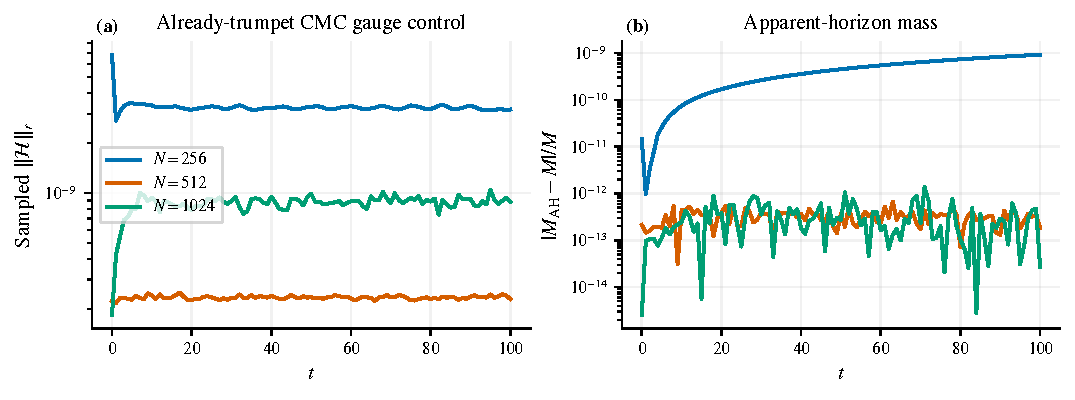
\includegraphics[width=\textwidth]{cmc_control}
 \caption{Already-trumpet CMC control, $M=1/3$, with an analytic CMC lapse source and reference-lapse damping. Sampled Hamiltonian RMS and relative apparent-horizon mass error remain small through $t=100$, but the finest Hamiltonian curve shows a floor/upturn. Isolated zero mass errors are omitted on the logarithmic axis. These data are neither wormhole-to-trumpet evolution nor the main Minkowski-reference gauge.}
 \label{fig:cmc}
\end{figure*}

\subsection{Genuine wormhole data and strong-field fronts}
\label{sec:wormhole}
The wormhole data are constructed as a slice of Schwarzschild spacetime rather than by compactifying time-symmetric data and assuming hyperboloidal asymptotics. With $F_S=1-2M/R$, prescribe the physical normal radius derivative $H(R)=s(R)R$, where the smooth outer-branch switch rises from zero at $4M$ to one at $8M$. Then
\begin{equation}
 \begin{gathered}
 h_R=\frac{H}{F_S\sqrt{F_S+H^2}},\quad
 \widetilde\gamma_{RR}=\frac1{F_S+H^2},\\
 K_R{}^R=-H_R,\quad K_\theta{}^\theta=-H/R.
 \end{gathered}
\end{equation}
The inner region remains the two-ended isotropic wormhole,
\begin{equation}
 R=\rho\left(1+\frac{M}{2\rho}\right)^2,\qquad
 \widetilde\alpha=\left(1+\frac{M}{2\rho}\right)^{-2}.
\end{equation}
An isotropic compactifying map gives $g=1$ and joins this interior to a hyperboloidal exterior. The second asymptotically flat end is excluded from the outer height transition. The construction is analytically vacuum; the recorded initial-data audit gives Hamiltonian and momentum errors below $2.3\times10^{-13}$ and $3.9\times10^{-14}$ at its tested points.

For $M=1/3$ and $\nu=1$, the modified logarithmic source still produces a sharp inward-moving front. At $t=2.5$, the physical-lapse gradient near $r=0.119$ increases from $22.86$ to $40.65$ to $76.92$ as $N$ increases from $513$ to $1025$ to $2049$. The trace develops a narrow negative spike, and local Hamiltonian maxima increase from $0.409$ to $0.654$ to $0.974$ (Fig.~\ref{fig:front}). The front subsequently moves inward. These data rule out a smooth, resolved convergence interpretation of that trial. They support a gauge-steepening diagnosis, but do not prove a gauge-shock theorem for this spherical, nonlocal-shift system. Results for simpler slicing systems\cite{Alcubierre2005,BaumgarteHilditch2022} motivate this interpretation without establishing it here.

\begin{figure*}[tp]
 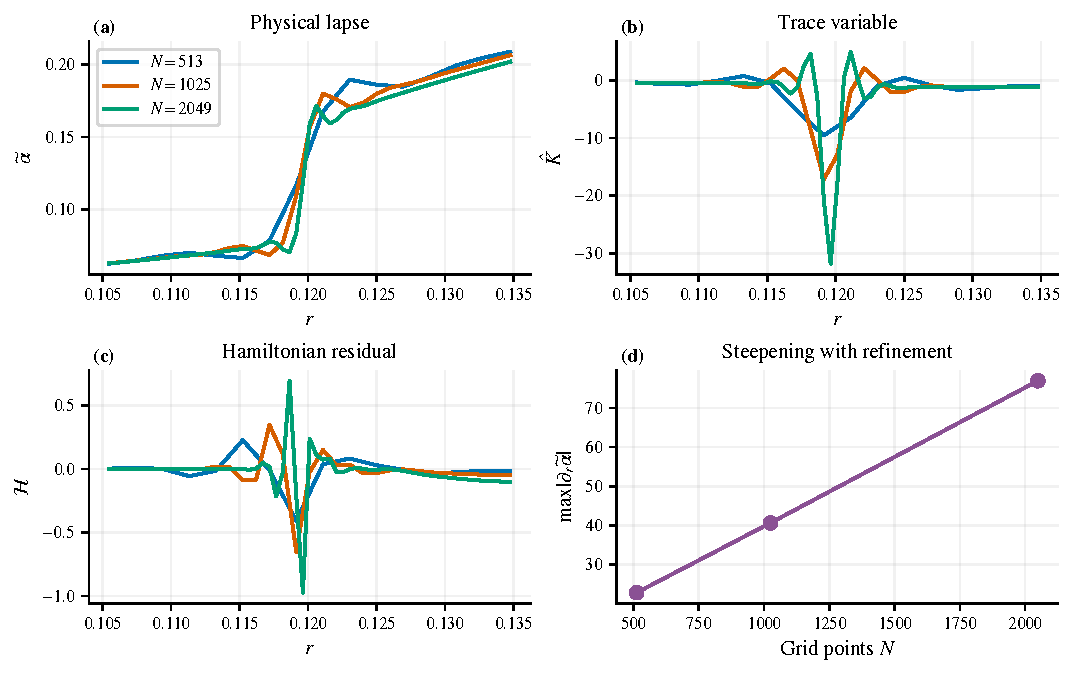
\includegraphics[width=\textwidth]{wormhole_front}
 \caption{Failed $\nu=1$ wormhole trial with the modified logarithmic source, shown at the exact saved time $t=2.5$. The physical lapse steepens, $\Kh$ develops a narrow spike, and the local Hamiltonian error grows under refinement. The gradient diagnostic in (d) uses second-order differentiation of saved profiles; it is not the evolution stencil. This is evidence of unresolved steepening, not a proof of a continuum shock.}
 \label{fig:front}
\end{figure*}

Reducing the positive logarithmic coefficient to $\nu=0.25$ improves the early evolution. Full-domain prefixes on $N=2049,4097,8193$ through $t=3.2$ give peak physical-field self-convergence orders $5.50$ in the bulk and $5.86$ near scri. The peak accepted momentum RMS decreases as $2.77\times10^{-5}$, $1.47\times10^{-6}$, and $6.87\times10^{-8}$. The Hamiltonian RMS, however, is $1.01\times10^{-7}$, $3.00\times10^{-9}$, and $5.37\times10^{-9}$; the finest upturn remains visible. These are prefix results only. An existing exact-source continuation of $N=4097$ reaches $t=3.6$, but does not supply the missing full long-duration study.

\subsection{Causal retained domains: improvement without acceptance}
The retained-domain comparison transfers the saved $t=3.2$ wormhole states to $r\geq1/64$, using the global profile in Eq.~\eqref{eq:trumpet-chart}. It retains $1009$, $2017$, and $4033$ points from full grids of $1025$, $2049$, and $4097$, respectively. The main gauge remains Minkowski-referenced, with $\nu=0.25$, the modified logarithmic source, and constant damping. All runs reach $t=10$ and remain outward-characteristic at the cutoff. Their transient constraint accuracy is insufficient (Table~\ref{tab:domain}).

\begin{table}[tbp]
\caption{Retained-domain peak accepted-state constraints on $3.2\leq t\leq10$. These maxima include the early transient.}
\label{tab:domain}
\begin{ruledtabular}
\begin{tabular}{rcc}
$N$ & $\max_t\normr{\HH}$ & $\max_t\normr{\MM}$\\
\hline
1009 & $5.45\times10^{-4}$ & $1.46\times10^{-3}$\\
2017 & $2.10\times10^{-4}$ & $5.25\times10^{-4}$\\
4033 & $4.63\times10^{-5}$ & $1.20\times10^{-4}$
\end{tabular}
\end{ruledtabular}
\end{table}

RMS Hamiltonian pair orders are approximately $1.38$ and $2.18$, with momentum orders $1.47$ and $2.12$. Bulk maximum-norm orders are lower still. Clean late-time constraints or an accurate exterior mass therefore do not establish a successful experiment. Figure~\ref{fig:domain} retains the transient and shows a distinct representation effect: the compact metric profile introduces late constraint structure near $r\simeq0.112$, inside its transition region. The same-grid global profile largely removes this artifact. The transient remains in both, so eliminating the profile artifact is not a complete repair.

The earlier finite-cutoff and asymptotic-chart failures also limit interpretation. An outward physical light cone alone was insufficient because the gauge cone could be incoming. A gauge-only Robin treatment later halted when a physical characteristic entered. Stronger dissipation, SBP6/3 differentiation, and a tapered cutoff filter did not produce an accepted full wormhole evolution. For finite time the full continuum wormhole retains an asymptotically flat inner core; a trumpet limit must be established outside that shrinking core using lapse collapse, limiting areal radius, proper-distance behavior, and invariant convergence. That demonstration remains unfinished.

\begin{figure*}[tp]
 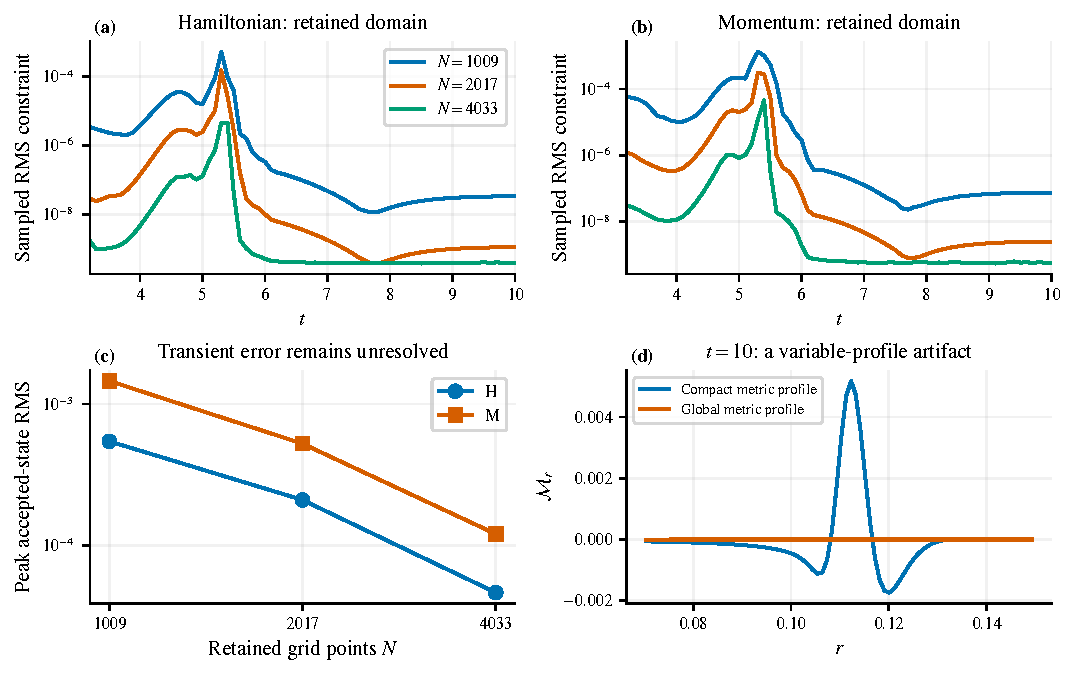
\includegraphics[width=\textwidth]{retained_domain}
 \caption{Completed retained-domain experiments with the global metric profile and $\nu=0.25$. Panels (a,b) show saved-time RMS constraints, whereas (c) uses maxima over every accepted state; narrow peaks can exceed the saved-time curves. The measured orders remain inadequate. Panel (d) isolates the late compact-profile artifact using two $N=1009$ runs with identical physical initial fields and gauge sources. These plots exclude the excised region and cannot replace assessment of the full preceding wormhole trajectory.}
 \label{fig:domain}
\end{figure*}

\subsection{Scalar propagation, dispersal, and failed collapse}
An independent fixed-Minkowski scalar solver provides a preliminary propagation oracle. The physical analytic solution is an ingoing/outgoing spherical wave of the form $\phi=[F(T-R)-F(T+R)]/R$. This separate second-order characteristic discretization gives weighted-field orders $1.96$ and $2.00$ and scri orders $1.90$ and $1.98$ on $N=200,400,800$ through $t=3$ [Fig.~\ref{fig:scalar}(a)]. It neither tests the full coupled geometry nor establishes high-order accuracy of the evolution code.

The coupled subcritical data use
\begin{equation}
 \phi(0,r)=A_\phi\exp\left[-\frac{(r^2-0.25^2)^2}{4(0.1)^4}\right],
 \qquad A_\phi=0.058,
\end{equation}
with the constraint solve described above. The initial mass is approximately $0.105734092466$. At $t=6$, $|M_0-E_{\rm rad}|$ is $6.99\times10^{-6}$, $2.53\times10^{-7}$, and $8.19\times10^{-9}$ on $N=512,1024,2048$. The residual mass sampled at $r=0.9$ is about $1.9\times10^{-11}$, much smaller than the finest budget discrepancy. The two budget-error ratios correspond to orders about $4.79$ and $4.94$.

The finest run has peak scri pole residue $1.26\times10^{-8}$ and a conservative nonaffinity bound $6\max|\kappa_B|=5.80\times10^{-8}$, below the specified $10^{-7}$ bound. The two coarser runs fail some boundary/affinity gates. We use the RK-integrated flux for this comparison: quadrature of sparsely saved flux samples can underresolve the pulse by much more than the reported budget error. The result is a short-time coupled dispersal check, not a measured tail or a completed principal study with all independent controls.

The collapse attempts are unsuccessful. The latest positive-variable, upwind, $A_\phi=0.07$ trial reaches $t=3$ at all three resolutions, but its all-stage Hamiltonian RMS peaks are $3.71\times10^8$, $3.05\times10^{10}$, and $1.94\times10^{10}$. Sampled histories are shown in Fig.~\ref{fig:scalar}(d). Numerical survival and any apparent-horizon crossing in such a trajectory cannot be interpreted as reliable black-hole formation. Earlier source and transport variants also failed. No coupled black-hole scalar perturbation, quasinormal frequency, or late-time decay exponent is extracted from these data. Those physical tests, including neutral limits of later scalar studies\cite{Alvares2026}, remain future work.

\begin{figure*}[tp]
 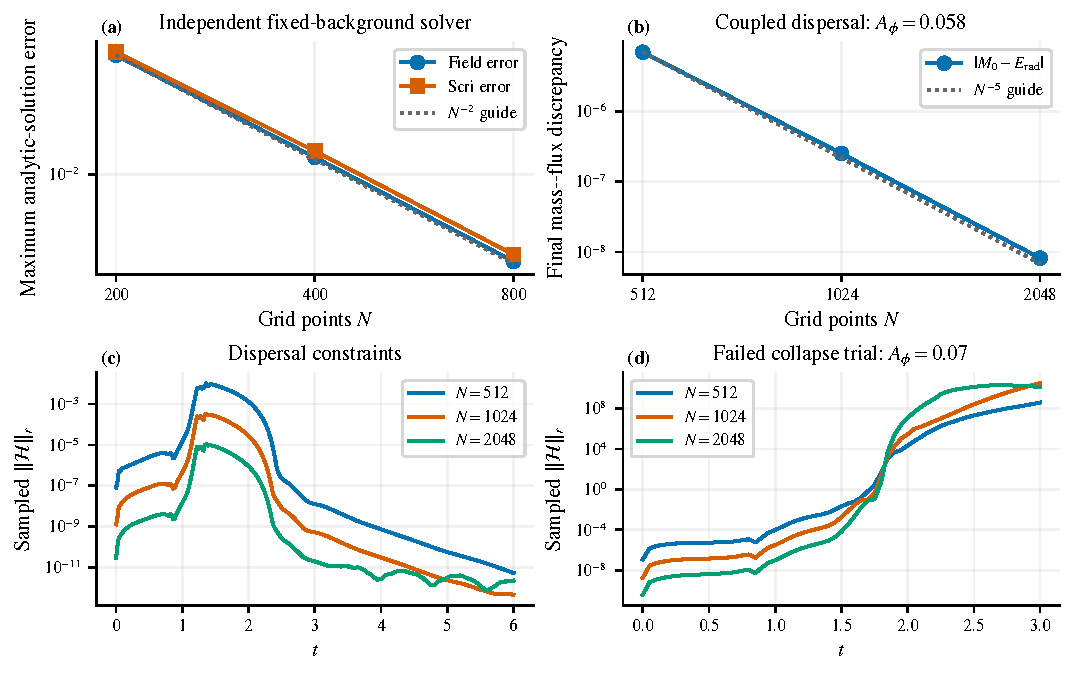
\includegraphics[width=\textwidth]{scalar_results}
 \caption{Scalar evidence with its scope kept explicit. (a) Independent second-order fixed-background oracle. (b) Coupled subcritical mass--flux discrepancy at $t=6$; the dotted slope is a guide. (c) Sampled coupled dispersal constraints. (d) A different, failed $A_\phi=0.07$ collapse family with enormous constraints. Panels (c,d) use different lapse-source/variable choices, so their contrast is not a controlled amplitude-only comparison. Reaching the target time in (d) is not evidence of accurate collapse.}
 \label{fig:scalar}
\end{figure*}

\section{Spherical conformal telegrapher follow-up}
\label{sec:telegraph}
The unresolved front in Fig.~\ref{fig:front} motivates a separate modification of the lapse gauge. This follow-up retains the full two-ended wormhole chart, the metric-derived elliptic shift, and independently evolved Z4c fields. It does not use the retained-domain transfer of the preceding section. In particular, neither the region inside the apparent horizon nor a neighborhood of the puncture is excised. The new numerical evidence is reported separately from the historical source and boundary trials.

\subsection{Relaxation equation and spherical coupling}
Set $D=\partial_t-\beta\partial_r$ and retain $u=\alpha-A$. We introduce a radial auxiliary component $B$ and a fixed taper $\varpi(r)$, with additions
\begin{align}
 \Delta(D\alpha)&=\chi\left[\varpi B_r+
 \left(\varpi_r+\frac{2\varpi}{r}\right)B\right],
 \label{eq:telegraph-alpha}\\
 \tau_T DB&=\kappa_T\varpi u_r-B.
 \label{eq:telegraph-B}
\end{align}
Here $B$ is unrelated to a shift-driver variable, and $\tau_T$ is unrelated to the endpoint penalty coefficient in Eq.~\eqref{eq:penalty}. The lapse addition equals $\chi r^{-2}\partial_r(r^2\varpi B)$. Its two angular terms follow from the flat-reference contraction of $B_i=B(r)x_i/r$. We retain componentwise advection of $B$ and divide Eq.~\eqref{eq:telegraph-alpha} by the total positive $\alpha$ when updating the logarithmic lapse variable. This is an explicit conformal coordinate gauge inspired by a telegrapher relaxation mechanism; it is not a covariant transformation of the Cartesian physical-lapse implementation. No Hamiltonian, momentum, or Z4 constraint is substituted into these equations.

The initial data have $B=0$. The selected taper is one for $r\leq0.56$, decreases smoothly to zero over $0.56<r<0.8$, and is zero for $r\geq0.8$. The transition uses the $C^7$ rational ramp $R_7(z)=z^8/[z^8+(1-z)^8]$, with $z=(0.8-r)/0.24$ clipped to $[0,1]$. This differs from the polynomial smoothstep used for the numerical grid map below. Consequently the direct addition vanishes near scri, preserving the existing clock and compatibility equations. An earlier version also set the coupling to zero in an inner collar; it lost effectiveness when the front entered that collar and is not the selected prescription.

Keeping $\varpi=1$ near the asymptotically flat end is regular. With $\chi=X_0r^4+O(r^5)$, $\alpha=a_2r^2+O(r^3)$, $\beta=b_1r+O(r^2)$, and $B=b_Br+O(r^2)$, Eq.~\eqref{eq:telegraph-B} gives
\begin{equation}
 \dot b_B=b_1b_B+\frac{\kappa_T(2a_2-1)-b_B}{\tau_T}.
\end{equation}
The added lapse rate is $3X_0b_Br^4+O(r^5)$, and the added logarithmic rate is $(3X_0b_B/a_2)r^2+O(r^3)$. Thus the leading AF lapse coefficient equation is unchanged. The endpoint condition $B(0)=0$ is preserved by its evolution; this argument uses AF asymptotics, not regular-center reflection parity.

\subsection{Characteristic speeds and the meaning of compression}
The frozen radial lapse--trace--flux subsystem has speeds
\begin{equation}
 c_0=-\beta,\qquad
 c_\pm=-\beta\pm\sqrt{\chi\left(F+\frac{\kappa_T\varpi^2}{\tau_T}\right)}.
\label{eq:telegraph-speeds}
\end{equation}
The shift and metric factors are essential. Using the isolated telegrapher speed alone would underestimate the coupled propagation speed. Define $c_g^2=\chi F$ and $c_T^2=\chi\kappa_T\varpi^2/\tau_T$. In the locally advected frame, the frozen Fourier dispersion polynomial is
\begin{equation}
 s^3+\frac{s^2}{\tau_T}+(c_g^2+c_T^2)k^2s
 +\frac{c_g^2k^2}{\tau_T}=0.
\label{eq:telegraph-dispersion}
\end{equation}
For nonzero $k$, positive $c_g^2,c_T^2$, and $\tau_T>0$, the Routh--Hurwitz inequality is strict. The high-frequency propagating pair has damping rate
\begin{equation}
 \gamma_\infty=\frac{c_T^2}{2\tau_T(c_g^2+c_T^2)}.
\end{equation}
These frozen-subsystem statements motivate the mechanism; they do not prove stability or shock avoidance for the nonlinear free-Z4c system with elliptic shift feedback.

For each family we evolve a ray position and a ray-map Jacobian $\mathcal J_\pm$,
\begin{equation}
 \dot r_\pm=c_\pm(t,r_\pm),\qquad
 \frac{\dd}{\dd t}\log\mathcal J_\pm=\partial_r c_\pm(t,r_\pm).
\label{eq:telegraph-rays}
\end{equation}
There are 81 matched seeds per family, uniformly spanning $0.12\leq r\leq0.4$, activated exactly at $t=1$. The stage geometry and stage elliptic shift supply the speed at every RK evaluation. A shape-preserving $C^1$ piecewise cubic Hermite interpolant supplies both the speed and its analytic derivative\cite{PCHIP}; it is applied only to passive diagnostics and cannot smooth the evolved lapse. Boundary exits are located using a continuous RK4 extension\cite{RK4Dense}; the terminal position and compression are evaluated at the same exit event and then frozen. The implementation also checks for an exit followed by a return within a step. Intermediate ray stages may continue the endpoint speed polynomial by at most one boundary-cell width; the geometry and elliptic equations are never evaluated outside the domain. Terminal coincidences at scri are not characteristic crossings.

For a regular Lipschitz finite-grid velocity, $\mathcal J=\exp(\int\partial_rc\,\dd t)$ stays positive. Finite-grid ray ordering therefore cannot prove continuum noncrossing. Conversely, a very small positive $\mathcal J$ is compression, not an observed intersection. The relevant evidence is joint spatial and temporal convergence of the lapse, its gradient, the constraints, and the ray diagnostics. The original unmodified gauge gave inward $\min\mathcal J$ at $t=3$ of $1.26\times10^{-5}$ and $1.22\times10^{-8}$ at $N=513$ and $1025$, respectively. This resolution-dependent compression supports the unresolved-steepening diagnosis, without importing a shock theorem from a simpler slicing system\cite{Alcubierre2005}.

\subsection{Mapped discretization and implementation checks}
The baseline is the modified logarithmic source of Eq.~\eqref{eq:physical-log}, with constant constraint damping. The selected parameters are $M=1/3$, $\nu=1$, $\kappa_T=0.005$, $\tau_T=0.02$, and $\Delta t=0.05\Delta x$, with $x_i=i/(N-1)$. All continuum equations remain expressed in $r$. A fixed numerical map resolves the shrinking inner layer:
\begin{equation}
 E(x)=\frac{\operatorname{expm1}(32x)}{2\operatorname{expm1}(16)}.
\end{equation}
It is used through $x=0.3$, joined to $r=x$ over $0.3<x<0.5$ by $r=(1-S)E+Sx$, and followed by the identity through $x=0.8$. For the inner join, $S=S_7((x-0.3)/0.2)$, where
\begin{equation}
 S_7(z)=\sum_{j=8}^{15}\binom{15}{j}z^j(1-z)^{15-j},
 \qquad 0\leq z\leq1.
\end{equation}
For $x>0.8$, let $L=0.2$ and $y=(x-0.8)/L$ and use
\begin{equation}
 r=x+\tfrac12Ly^8(1-y),\qquad
 J_x\equiv\frac{\dd r}{\dd x}=1+\tfrac12y^7(8-9y).
\end{equation}
This join is $C^7$, monotone, fixes actual scri, and gives $J_x(1)=1/2$. It refines the outer endpoint without changing the inner map. Derivative and interval-quadrature weights are constructed on the actual $r_i$; the endpoint penalty spacing is $\Delta xJ_x(1)$. The map is fixed across resolution, and no physical nodes are removed.

The selected implementation retains seven-point derivative stencils and seven-point shift quadrature. It replaces sixth-difference dissipation by eighth-difference dissipation. Writing $D_p$ for the unscaled $p$th forward difference, the mapped filter is
\begin{align}
 Q_{2p}&=-\frac{\epsilon}{2^{2p}\Delta x}
 J_x^{-1}D_p^T\operatorname{diag}(W\overline J)D_p,\\
 \overline J_i&=\frac{p+1}{\sum_{j=0}^{p}1/J_{x,i+j}},\qquad p=4,
\end{align}
with $\epsilon=0.5$ and the existing nonnegative physical-radius taper $W$. The AF coefficient column is excluded from this filter, while its continuum endpoint ODE is still evolved. Geometry and $B$ use the same filter. Its discrete $J_x$-weighted energy contribution is nonpositive and its smooth interior truncation contribution is $O(\Delta x^7)$. The isolated-filter guard is $\Delta t\epsilon/\Delta x\leq2/(p+1)$; characteristic and relaxation guards are also enforced. These properties do not provide a stability estimate for the combined nonlinear operator.

On this map, the full-grid constraint RMS is
\begin{equation}
 \normr{C}=\left[\frac{\sum_i r_i^2J_{x,i}C_i^2}
 {\sum_i r_i^2J_{x,i}}\right]^{1/2}.
\label{eq:telegraph-norm}
\end{equation}
It uses the implemented conformal constraint quantities and is not a proper-volume norm. It downweights the near-puncture region and gives zero weight to the endpoint $r=0$, so we also retain unweighted pointwise maxima on the full grid and on $0\leq r<0.8$. The latter cutoff removes the outer region toward scri, not the black-hole interior. No differential constraint is projected, reset, or masked in the acceptance assessment.

The implementation checks include independent nonzero-flux Python/compiled rates, spherical angular contractions, free-constraint RK stages, exact zero-flux regression, mapped differentiation/quadrature, filter energy identities, stage rays, and compensated-state restart. The complete 55-group suite passed after the dense-exit implementation. A subsequent analysis-only change passed its two targeted CTest groups; it is not described as a rerun of the expanded 56-group suite. Pure exit-event oracles showed approximately fourth-order errors, whereas the actual $C^1$ interpolated speed requires its own measured timestep study.

\subsection{Completed spatial experiment and measured limitations}
\newcommand{\TeleBulkOrder}{5.89}
\newcommand{\TeleEndpointOrder}{5.63}
\newcommand{\TeleHOrder}{6.52}
\newcommand{\TeleMOrder}{6.48}
\newcommand{\TeleThetaOrder}{6.62}
\newcommand{\TeleZOrder}{6.49}
\newcommand{\TeleGradientPercent}{0.103}
\newcommand{\TeleSpatialAssessment}{All listed spatial, boundary, and positivity checks pass for this fixed candidate. This is a finite-duration spatial result, not completion of the independent-control protocol.}
\newcommand{\TeleFinalHMax}{\ensuremath{2.290\times10^{-5}}}
\newcommand{\TeleFinalHRadius}{\ensuremath{1.465\times10^{-6}}}
\newcommand{\TeleAHMassError}{\ensuremath{1.267\times10^{-10}}}
\newcommand{\TeleRayGap}{\ensuremath{8.323\times10^{-11}}}
\newcommand{\TeleRayPositionError}{\ensuremath{6.209\times10^{-9}}}
\newcommand{\TeleRayLogError}{\ensuremath{5.507\times10^{-6}}}
\newcommand{\TeleMSMassError}{\ensuremath{1.476\times10^{-4}}}
\newcommand{\TeleAFMassError}{\ensuremath{2.916\times10^{-6}}}
\newcommand{\TeleMinLogJ}{-17.554446}
\newcommand{\TeleRayPositionOrder}{4.72}
\newcommand{\TeleRayLogOrder}{3.59}

The three related grids $N=1025,2049,4097$ reach $t=10$ with identical continuum parameters, numerical map, CFL factor, derivative width, and dissipation amplitude. This includes the complete initial transient and late inward compression. The comparison uses exact common physical nodes and 201 saved times; the constraint and boundary maxima in Table~\ref{tab:telegraph} are accumulated over every accepted state or every checked stage, as appropriate, rather than inferred only from those snapshots.

\begin{table}[tbp]
\caption{Full-duration telegrapher results on $0\leq t\leq10$. The Hamiltonian columns are maxima over accepted states; the pole column is the maximum checked scri residue. The pointwise Hamiltonian column includes $0\leq r<0.8$, retaining the puncture neighborhood.}
\label{tab:telegraph}
\begin{ruledtabular}
\small
\setlength{\tabcolsep}{3pt}
\begin{tabular}{rccc}
$N$ & $\max_t\normr{\HH}$ & $\max_{t,r<0.8}|\HH|$ & Scri pole\\
\hline
1025 & $5.401\times10^{-5}$ & $8.121\times10^{-2}$ & $2.833\times10^{-6}$\\
2049 & $1.405\times10^{-6}$ & $2.238\times10^{-3}$ & $1.414\times10^{-7}$\\
4097 & $1.528\times10^{-8}$ & $2.290\times10^{-5}$ & $4.212\times10^{-9}$

\end{tabular}
\end{ruledtabular}
\end{table}

The peak-in-time field-difference orders are \TeleBulkOrder\ in the bulk and \TeleEndpointOrder\ near scri. The finest-pair orders of the accepted-state RMS maxima for $(\HH,\MM,\Th,Z_r)$ are $(\TeleHOrder,\TeleMOrder,\TeleThetaOrder,\TeleZOrder)$. The maximum matched lapse-gradient discrepancy, normalized separately at each time by the fine-grid peak on common nodes, is \TeleGradientPercent\ percent. The original thresholds are unchanged: bulk field and constraint order at least $3.5$, endpoint field order at least $3$, finest Hamiltonian RMS below $10^{-5}$, pointwise Hamiltonian below $10^{-3}$ on $r<0.8$, and matched gradient discrepancy below $10\%$. \TeleSpatialAssessment

Figures~\ref{fig:tele-lapse} and \ref{fig:tele-resolution} show that an inward-moving nonmonotone lapse structure remains. Its survival as a profile feature is not itself a convergence failure: the relevant questions are whether its amplitude, width, derivatives, and associated constraints stabilize under refinement. Conversely, close agreement of two lapse curves alone is insufficient. By $t=10$ the physical-lapse structure occupies radii of order $10^{-6}$, which motivates the fixed exponential grid. A large coordinate derivative in this shrinking region is not, by itself, proof of a continuum discontinuity.

\begin{figure*}[tp]
 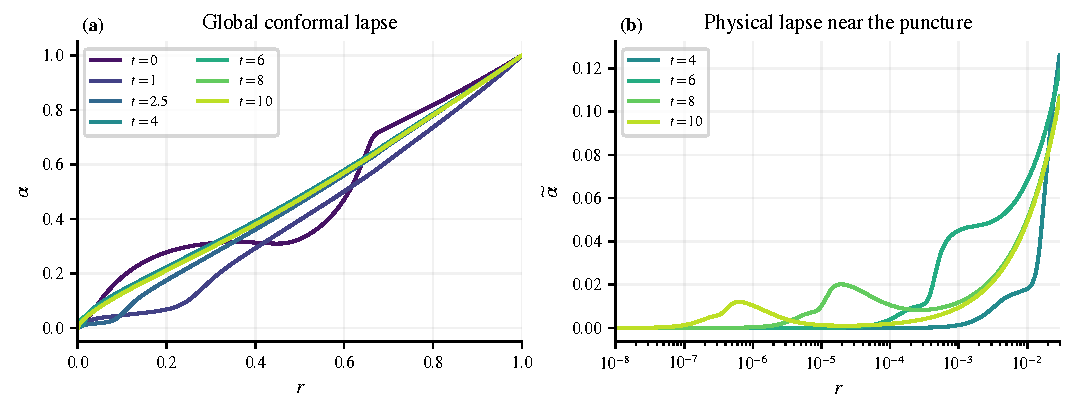
\includegraphics[width=\textwidth]{telegraph_lapse_evolution}
 \caption{Telegrapher lapse evolution on the finest completed grid, $N=4097$. The global panel uses conformal $\alpha$, which remains finite at scri. The inner panel uses physical $\widetilde\alpha=\alpha/\Omega$ and logarithmic radius to expose the late nonmonotone structure. Curves use saved profiles without smoothing or temporal interpolation. The remaining bump is not declared eliminated.}
 \label{fig:tele-lapse}
\end{figure*}
\begin{figure*}[tp]
 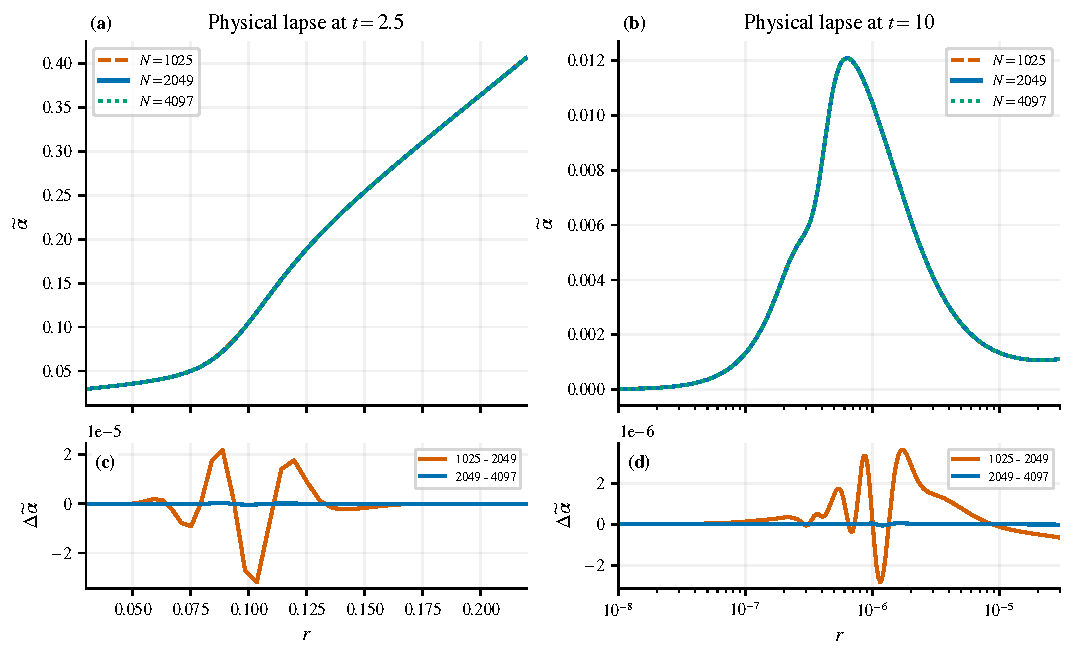
\includegraphics[width=\textwidth]{telegraph_lapse_resolution}
 \caption{Three-grid physical-lapse comparison at $t=2.5$ and $t=10$. The lower panels show raw consecutive-grid differences at matching physical nodes. The late panel retains the near-puncture structure instead of cutting it out. These are profile comparisons; whole-trajectory derivative and constraint checks are reported separately.}
 \label{fig:tele-resolution}
\end{figure*}

Figure~\ref{fig:tele-constraints} presents all four constraint histories. The radial RMS can be small while a sharply localized inner error is appreciable. At $t=10$ on $N=2049$, for example, $\normr{\HH}=9.67\times10^{-8}$ but $\max_r|\HH|=2.24\times10^{-3}$. That peak lies at $r=1.46\times10^{-6}$, well inside the apparent horizon at $r=0.10765$; the exterior maximum is $1.05\times10^{-7}$. This is a localization diagnostic, not an exterior-only acceptance rule. On the finest grid, the corresponding final full-grid maximum is \TeleFinalHMax\ at $r=\TeleFinalHRadius$, and the peak sampled apparent-horizon mass error over the full run is \TeleAHMassError. The maximum sampled finite-node Misner--Sharp mass discrepancy over the same trajectory is \TeleMSMassError, including the near-scri and inner nodes; the maximum sampled AF-end coefficient-mass discrepancy is \TeleAFMassError. The actual scri mass slot is undefined in this diagnostic and is not included in that finite-node maximum. Neither small exterior error nor accurate horizon mass overrides an inner constraint failure. Figure~\ref{fig:tele-inner} makes the pointwise error, growing lapse gradient, error location, and mass diagnostic visible together.

\begin{figure*}[tp]
 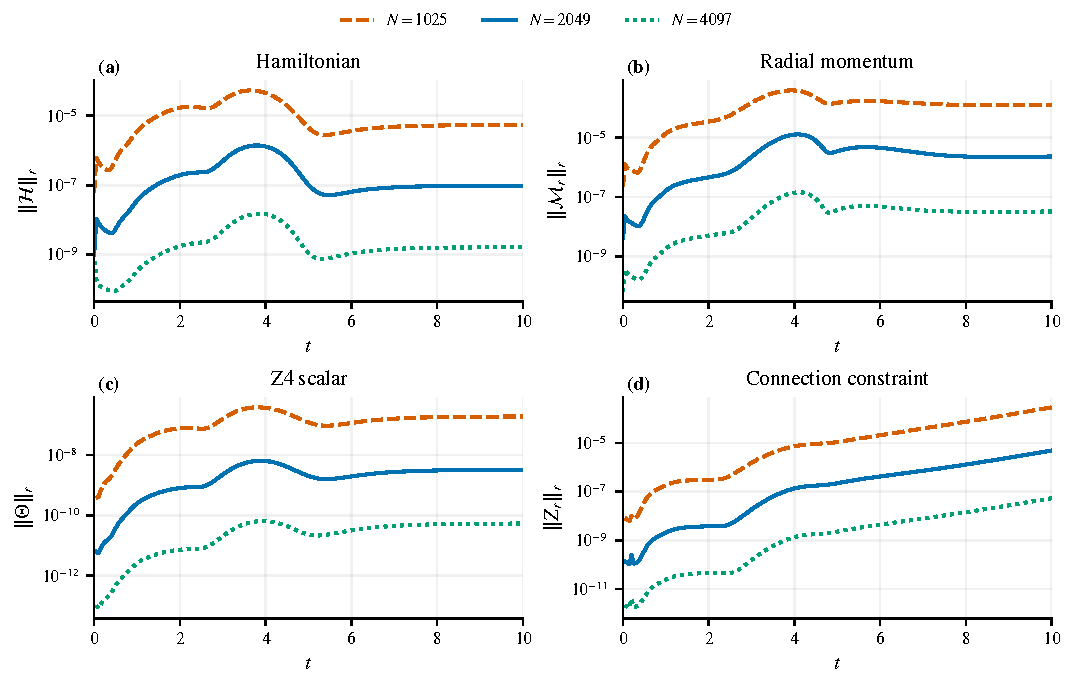
\includegraphics[width=\textwidth]{telegraph_constraints}
 \caption{Full-domain radial RMS constraints for the completed telegrapher sequence, using Eq.~\eqref{eq:telegraph-norm}. Every plotted value was recomputed from saved fields and checked against the recorded history. These curves sample every $0.05$ time units; the accepted-state maxima in Table~\ref{tab:telegraph} can be slightly larger. No interior mask is applied. The radial weighting suppresses small-radius contributions, so Fig.~\ref{fig:tele-inner} also reports the full-grid pointwise Hamiltonian error.}
 \label{fig:tele-constraints}
\end{figure*}
\begin{figure*}[tp]
 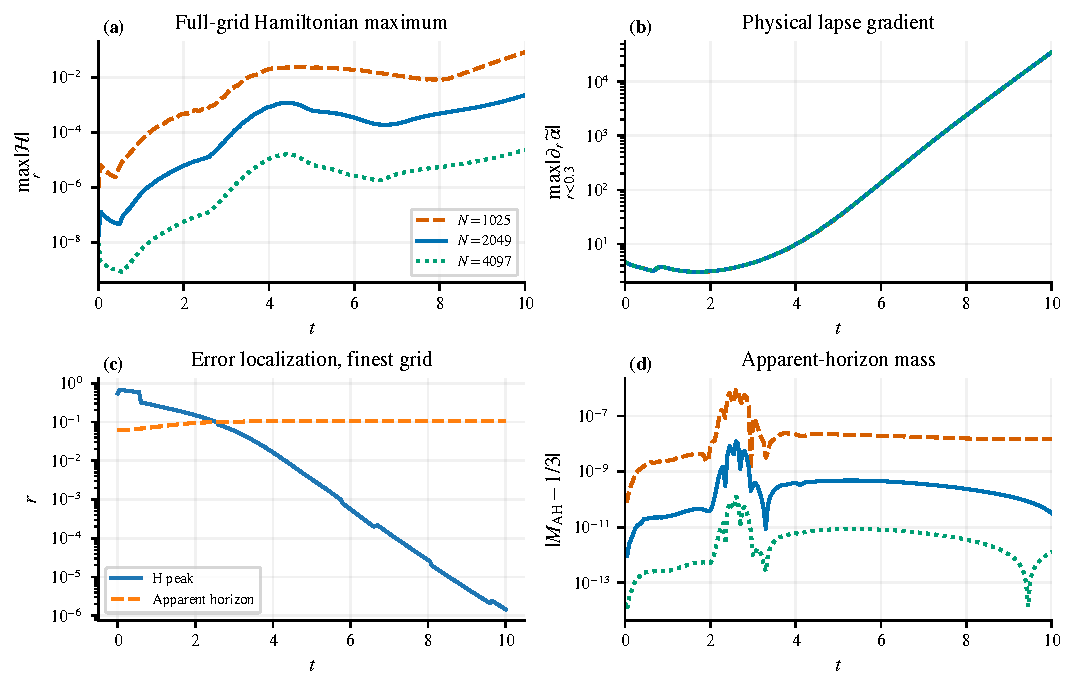
\includegraphics[width=\textwidth]{telegraph_inner_errors}
 \caption{Diagnostics that prevent a small radial RMS from hiding the inward layer. (a) Unweighted full-grid Hamiltonian maximum. (b) Physical-lapse gradient over $0\leq r<0.3$, evaluated with analytic AF factors and seven-point chart derivatives. (c) Position of the finest-grid Hamiltonian peak compared with the apparent horizon. (d) Independent apparent-horizon mass error. The horizon is identified from the outgoing expansion; this does not locate the event horizon. Mass errors near floating-point precision do not establish an asymptotic order.}
 \label{fig:tele-inner}
\end{figure*}

The tracked rays retain their ordering in the sampled spatial comparison. At $t=10$, all 81 inward rays remain active and all 81 outward rays have exited at scri. The finest minimum active inward $\log\mathcal J_-$ is \TeleMinLogJ, and the minimum active neighboring-ray separation is \TeleRayGap. The maximum middle-to-fine differences over the full trajectory are \TeleRayPositionError\ in ray position and \TeleRayLogError\ in $\log\mathcal J$, including terminal states. The observed peak-difference orders are \TeleRayPositionOrder\ and \TeleRayLogOrder, respectively. Figure~\ref{fig:tele-rays} shows the ray fans, compression, and refinement differences. These measurements describe strongly compressed finite-grid characteristics; they do not establish a continuum intersection or its absence.

\begin{figure*}[tp]
 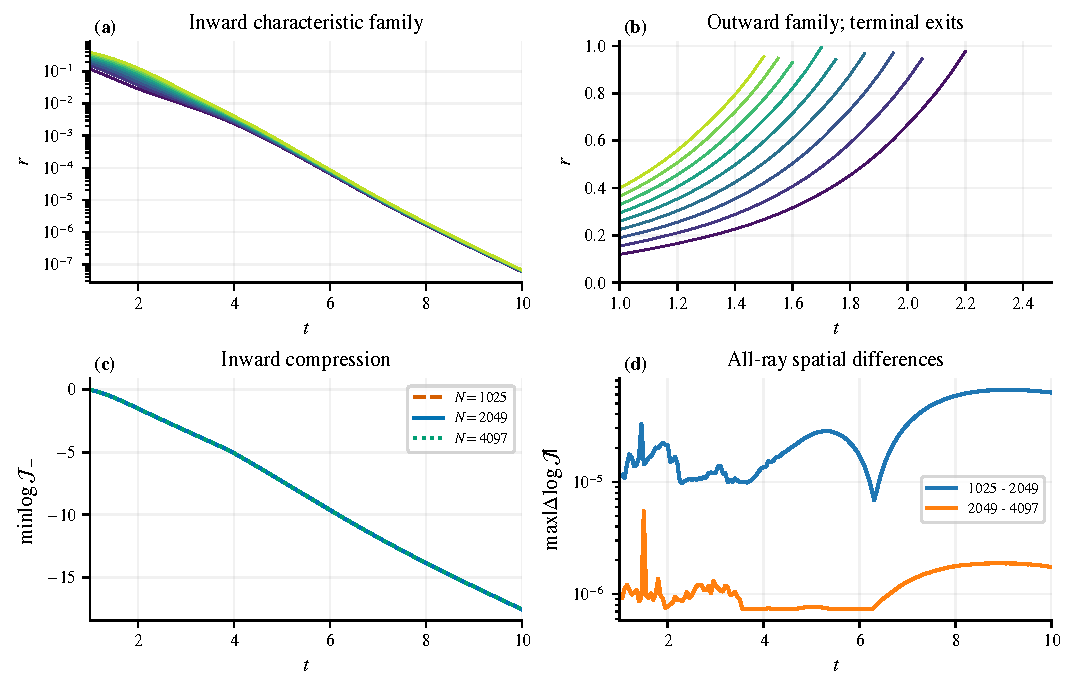
\includegraphics[width=\textwidth]{telegraph_characteristics}
 \caption{RK-stage characteristic tracking with matched dense exit events. The upper panels show nine representative seeds from each of the 81-ray families on $N=4097$. The outward panel zooms to the exit interval. Paths end at the last saved active point; no precise event time is fabricated from the plotting cadence. The lower-left panel shows inward compression across resolutions. The lower-right comparison includes all rays, including their frozen terminal compression. Positive finite-grid Jacobians and ordered rays are not a continuum shock-avoidance proof.}
 \label{fig:tele-rays}
\end{figure*}

\subsection{Independent timestep evidence at the stopping point}
The baseline and independent half-step $N=2049$ trajectories both reach $t=10$. The quarter-step control was paused at the requested finest-grid stopping point, with saved reports through $t=8.35$. Consequently the required full-duration three-level temporal-order and timestep-to-spatial-error assessment remains incomplete. The completed baseline--half-step comparison gives maximum bulk and endpoint field differences of $4.04\times10^{-12}$ and $2.33\times10^{-12}$, a Hamiltonian pointwise difference of $5.71\times10^{-10}$, and ray-position and $\log\mathcal J$ differences of $4.27\times10^{-13}$ and $7.68\times10^{-8}$. Two timestep levels alone do not establish temporal order. These raw differences, and the earlier short diagnostic pilot, cannot replace the missing robustness controls.



\subsection{Long-duration puncture pilot: exterior accuracy and termination}
\label{sec:tele-long}
A separate low-resolution continuation targeted $t=500$ on $N=1025$, starting from the verified $t=10$ checkpoint of the genuine wormhole trajectory. The frozen numerical source, binaries, map, CFL factor, relaxation parameters, and full-domain boundary treatment were unchanged. The run stopped at $t=43.836474609375$ with the native error \code{g=1 gauge or positivity violation}. Figure~\ref{fig:tele-long} reports all validated saved states through $t=43.8$, including the parent trajectory. The requested duration was not reached. This is a single-grid survival pilot, not an additional convergence study.

For this long-duration pilot we assess an apparent-horizon-exterior error budget and take apparent-horizon mass conservation as the primary invariant check. At each saved time, let $E(t)=\{i:r_i\geq r_{\rm AH}(t)\}$, where the existing outgoing-expansion finder locates $r_{\rm AH}$. With the same mapped radial weights $w_i=r_i^2(\dd r/\dd x)_i$ used previously, define
\begin{equation}
 \|C\|_{r,E}^2=\frac{\sum_{i\in E(t)}w_i C_i^2}{\sum_{i\in E(t)}w_i},
 \qquad C\in\{\HH,\MM,\Th,Z_r\}.
 \label{eq:exterior-norm}
\end{equation}
The pointwise budget uses $\max_{i\in E(t)}|C_i|$. Interior errors and puncture-end mass estimates are excluded from this budget. The normalization uses only exterior weights, rather than filling the excluded interior with zeros. This is a diagnostic selection: the evolution still includes every puncture-interior node. The historical three-grid full-domain assessment through $t=10$ remains unchanged and is labeled separately.

At the last saved time $t=43.8$, the exterior RMS values for $(\HH,\MM,\Th,Z_r)$ are $(1.79\times10^{-7},2.44\times10^{-6},5.00\times10^{-8},5.21\times10^{-7})$. The exterior Hamiltonian maximum is $5.88\times10^{-6}$. These late values remain nearly unchanged from $t=10$. The initial transient remains in the budget: the maximum sampled exterior Hamiltonian and momentum RMS values on $0\leq t\leq43.8$ are $1.84\times10^{-5}$ and $4.92\times10^{-5}$. The apparent-horizon mass error is $3.93\times10^{-8}$ at $t=43.8$, or $1.18\times10^{-7}$ relative to $M=1/3$; its peak sampled absolute error over the whole interval is $8.79\times10^{-7}$, corresponding to relative error $2.64\times10^{-6}$. The late mass error grows gradually while remaining below the initial-transient peak.

The saved exterior diagnostics do not show a blow-up before termination. Nevertheless, excluding interior diagnostic errors does not disable the full-domain evolution guard. The termination checkpoint remains finite, its metric deviation is exactly zero, and reconstructed lapse and conformal factor are positive at positive-radius nodes. The generic guard message does not preserve the offending stage or radial index. An offline replay, described below, localizes the failure to lapse underflow at the second positive-radius node during RK stage four. Puncture-interior constraints and mass estimates remain archived diagnostics and are excluded from the exterior budget. The result supports preserved horizon mass and a nearly steady late exterior constraint budget through the last saved profile, but does not establish survival to $t=500$ or exterior convergence. The failed trajectory is retained; the following floor controls are separate experiments.

\begin{figure*}[tp]
 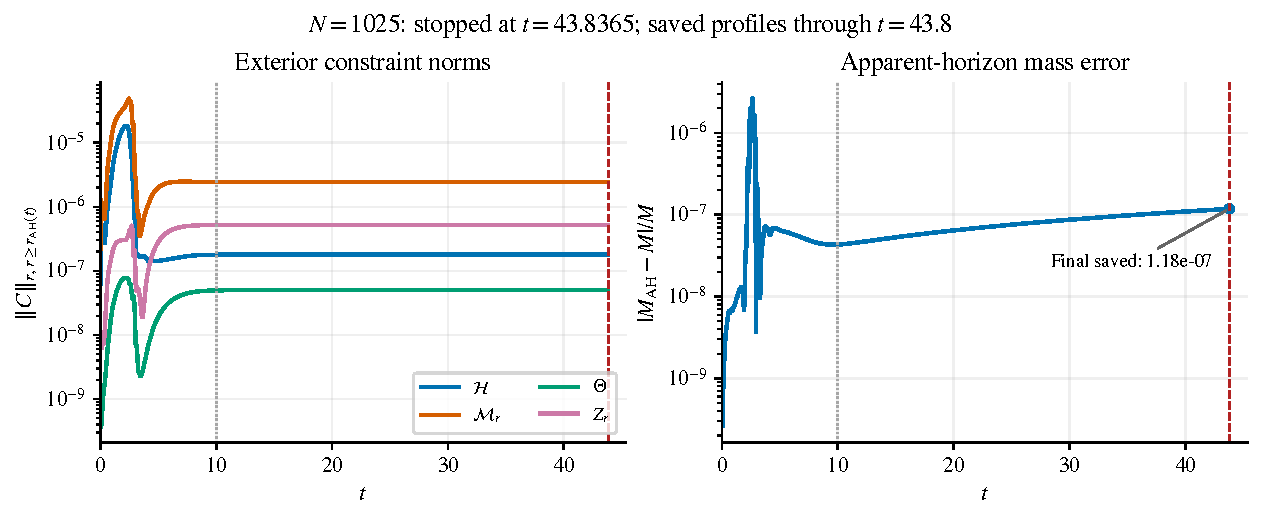
\includegraphics[width=\textwidth]{telegraph_long_exterior_status}
 \caption{Final saved history of the $N=1025$ puncture continuation targeting $t=500$. Left: apparent-horizon-exterior radial RMS constraints, normalized over the exterior region at each saved time. Right: relative apparent-horizon mass error, the primary invariant in the revised long-run budget. The gray dotted line marks the verified restart at $t=10$; the red dashed line marks the native guard stop at $t=43.8365$. Curves end at the last saved time $t=43.8$ and are not extrapolated to the failed stage. Puncture-interior errors and puncture mass estimates do not enter this budget. All 877 distinct saved profiles were checked for finite fields, reconstructed full-domain norms, and independently recomputed apparent horizons before evaluating the exterior diagnostics.}
 \label{fig:tele-long}
\end{figure*}


\subsection{Localized lapse underflow and a configurable floor}
\label{sec:lapse-floor}
Replaying the failed step on an isolated checkpoint copy with its frozen kernels reproduces the native rejection without advancing the original trajectory. At the second positive-radius node, $r=3.63\times10^{-9}$, the conformal lapse falls from $5.20\times10^{-11}$ at stage one to $1.25\times10^{-11}$ and $1.37\times10^{-13}$ at stages two and three. The fourth-stage value has $\log\alpha=-1109.3$, so reconstruction underflows to zero. The metric deviation remains zero and the conformal factor remains positive. The telegrapher contribution to the logarithmic lapse rate is approximately $-5.87\times10^4$, $-2.44\times10^5$, and $-2.22\times10^7$ in the first three stages, whereas the base-gauge contribution is positive and only of order $10^2$. Thus the additive flux contribution divided by the collapsing lapse drives the immediate rejection. Figure~\ref{fig:lapse-stop} shows the increasingly irregular inner profile and the replayed stage values.

We added the user-configurable input \code{lapse_floor}, with default $10^{-10}$ and $0$ to disable it. The CLI spelling is \code{--lapse-floor}. At ordinary nodes $0<r<1$, the numerical update applies
\begin{equation}
 \widetilde\alpha_i\leftarrow\max(\widetilde\alpha_i,\alpha_{\min}),
 \qquad \alpha_{\min}=10^{-10}\quad\hbox{by default},
\end{equation}
before each RK stage and after every accepted step, including initialization before the first report. The projection is implemented in the logarithmic lapse chart with an upward rounding margin. Only the clipped accepted lapse components have their compensated-update remainder reset. The AF coefficient endpoint and scri clock are unchanged; no constraint or other geometric field is projected. This is a finite-grid regularization of the unresolved interior, not an established continuum AF-end prescription. Historical inputs are explicitly pinned to zero floor, and the selected value is included in restart validation.

The native implementation with zero floor still reproduces the original rejection. With $\alpha_{\min}=10^{-10}$, a separate checkpoint control completes 20\,480 steps, one additional time unit, to $t=44.8365$. Only the first two positive-radius nodes require clipping in this control. Its final relative apparent-horizon mass error is $1.20\times10^{-7}$ and its exterior Hamiltonian RMS is $1.79\times10^{-7}$. Preliminary isolated controls with floors $10^{-8}$ and $10^{-6}$ also complete one time unit; these short controls do not establish long-duration stability. Seven targeted telegrapher test groups pass, including independent projected-RK comparison, preserved endpoint slots, disabled and invalid inputs, and exact floor-bound checkpoint restart. A separate fresh $N=1025$ wormhole trial with the default floor also targeted $t=500$. Its terminal outcome is reported below, separately from the unfloored failure and the completed three-grid study.

\begin{figure*}[tp]
 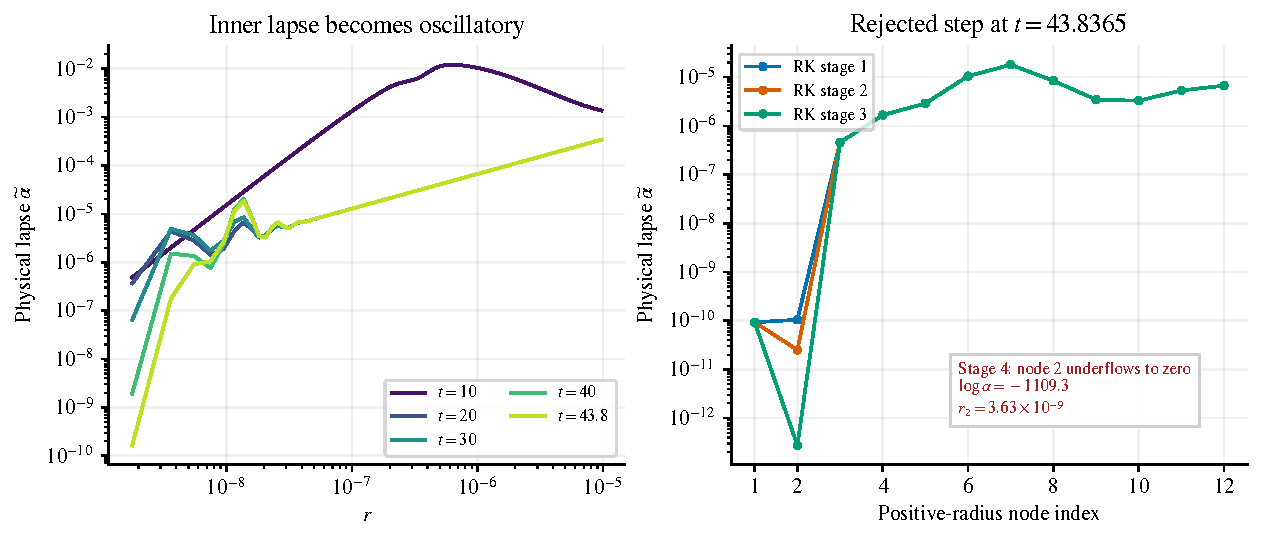
\includegraphics[width=\textwidth]{telegraph_lapse_stop}
 \caption{Diagnosis of the unfloored termination. Left: raw physical-lapse profiles in the innermost resolved region, showing irregular structure concentrated near the first few grid points. Right: the first three stages of an offline replay of the rejected step, using the frozen original kernels. Node two reaches $\log\alpha=-1109.3$ at stage four and underflows to zero; that zero is stated rather than plotted on the logarithmic axis. This local failure occurs far inside the apparent horizon. The floor controls are separate numerical experiments and do not overwrite this evidence.}
 \label{fig:lapse-stop}
\end{figure*}


\subsection{Terminal outcome of the floored duration trial}
\label{sec:floored-long}
The fresh wormhole trial with $\alpha_{\min}=10^{-10}$ stops at $t=84.798291015625$, after 1\,736\,669 accepted steps, with the native error \code{telegraph coupled-speed/relaxation timestep guard}. All 1696 saved profiles through $t=84.75$ were validated with the same source-binding, field-finiteness, full-domain-norm, and independent horizon checks used for the unfloored export. The original failed trajectory is preserved; this trial begins at $t=0$ with the floor applied to the analytic pre-collapsed lapse.

Figure~\ref{fig:floored-long} separates the exterior budget from the unresolved inner behavior. At $t=84.75$, the exterior RMS values for $(\HH,\MM,\Th,Z_r)$ are $(1.79\times10^{-7},2.44\times10^{-6},5.00\times10^{-8},5.21\times10^{-7})$, nearly unchanged from their late unfloored values. The exterior Hamiltonian maximum is $5.88\times10^{-6}$. The final saved apparent-horizon mass error is $7.01\times10^{-8}$, or $2.10\times10^{-7}$ relative to $M=1/3$. The maximum sampled relative error, $2.64\times10^{-6}$, still occurs during the initial transient. The last saved scri pole residue is $4.59\times10^{-13}$, with zero clock and nullness residuals. These statements apply to saved states, not to a successful continuation through the rejected step.

The floor remains localized far inside the apparent horizon: its outermost activation over the trajectory is $r=6.29\times10^{-7}$, compared with $r_{\rm AH}\simeq0.10765$. Nevertheless, the maximum upward correction to the stored lapse logarithm grows to $5.25\times10^3$ by the last saved state and $1.20\times10^4$ in the terminal diagnostics. This is substantial numerical clipping, rather than a uniformly small perturbation. The lower bound prevents lapse underflow but does not bound the independently evolved geometry or the elliptic shift.

An isolated replay with the exact frozen kernels reproduces the guard at the first stage of the next attempted step. The maximum occurs at positive-radius node three, $r=5.53\times10^{-9}$, where the physical lapse remains $10^{-10}$ but the reconstructed shift is $\beta^r\simeq3.93\times10^7$. Both coupled characteristic speeds are approximately $-3.93\times10^7$: shift transport dominates their splitting. With the mapped Jacobian $\dd r/\dd x=1.98\times10^{-6}$ and $\Delta t=4.8828125\times10^{-5}$, the checked mapped Courant number is $9.94\times10^{11}$, exceeding the limit $0.4$. The relaxation ratio remains $\Delta t/\tau=0.0024414$, so the speed condition triggers this guard. The last saved accumulated Courant maximum was only $0.2000$; the terminal event is not inferred by extrapolating that sampled history. The replay changes neither parameters nor timestep and does not continue the failed trajectory. Subsequent fresh repair trials are assessed separately in Sec.~\ref{sec:tele-repair-evidence}. The evidence establishes a later discrete inner failure despite a preserved saved exterior budget, not survival to $t=500$, continuum shock formation, or convergence of the floor prescription.

\begin{figure*}[tp]
 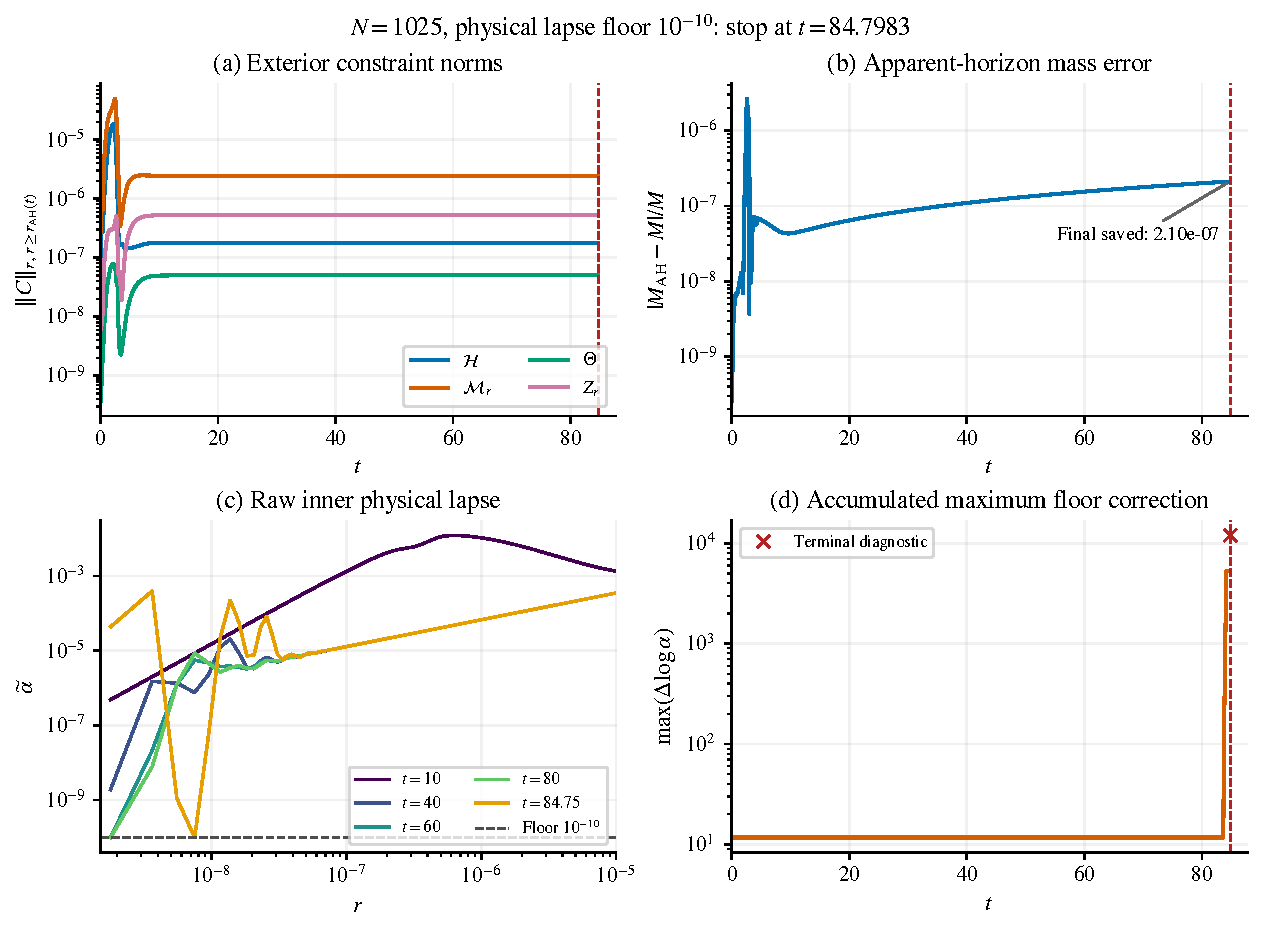
\includegraphics[width=\textwidth]{telegraph_floored_long}
 \caption{Separate fresh wormhole trial with physical lapse floor $10^{-10}$. (a) Apparent-horizon-exterior RMS constraints. (b) Relative apparent-horizon mass error. These primary diagnostics retain the complete initial transient and exclude the horizon interior. (c) Raw inner physical-lapse profiles, with the imposed floor marked; no smoothing is applied. (d) Accumulated maximum upward correction to the stored lapse logarithm, with the terminal diagnostic marked separately from the saved histories. The vertical red lines mark the speed-guard stop at $t=84.7983$; saved histories end at $t=84.75$. Large interior clipping is disclosed but is not substituted for the requested exterior error budget.}
 \label{fig:floored-long}
\end{figure*}


\subsection{Unsuccessful repairs and limits of the follow-up}
The refinement strategy was selected through documented failures. The inner-collar coupling lost influence after the front entered the collar; retaining the AF-regular coupling addressed that mechanism. Uniform and insufficiently clustered grids then underresolved the shrinking layer. A global clustering map improved inner resolution while degrading scri, motivating a map that preserves outer resolution. Increasing the differentiation width from seven to nine points produced a severe scri failure: the $N=513$, $t=6$ pilots had pole residues of order $5.6\times10^3$ and Hamiltonian RMS of order $0.20$, despite reaching their target time. A restricted outer-block spectrum supported a discrete-boundary explanation, but did not prove stability of the full system. Width seven was retained.

The previous KO6 exponential-map sequence met the inner spatial constraint magnitude and convergence gates through $t=10$ but missed the scri pole threshold: its finest residue was $1.0504\times10^{-7}$ against $10^{-7}$. Its old linear-ray/terminal-exit treatment also failed the independent compression accuracy criterion, with a timestep-to-spatial difference ratio of $0.2544$. Replacing only the speed interpolant by PCHIP did not cure terminal-event error. In the subsequent short pilot, adding matched dense exit events reduced the all-ray compression difference from $1.49\times10^{-4}$ to $9.89\times10^{-7}$ and its timestep-to-spatial ratio to $0.00168$. The saved geometry and auxiliary-flux histories were byte-identical across this diagnostic change. These were repairs to characteristic measurement, not an additional lapse-smoothing mechanism.

The current study ends at the requested finest-grid milestone. Independent shift-quadrature refinements, KO-amplitude variations, and adjacent fixed $\kappa_T,\tau_T$ three-grid controls were prepared but not executed. Their absence prevents a claim of robust parameter-independent convergence. Neither the telegrapher modification nor a successful finite-duration convergence check establishes a stationary trumpet limit, nonlinear shock avoidance for arbitrary data, or the missing scalar-collapse and radiation results.

\section{Failure analysis and limitations}
\label{sec:failures}
The negative results have changed both the implementation and the interpretation of apparently successful runs. Table~\ref{tab:failures} groups the principal failure mechanisms and unsuccessful repairs. A machine-readable supplement inventories 85 saved manifests with explicit failure status, including historical prototypes and deliberately rejected implementation fixtures. That count is not a count of independent physical experiments. Scientifically unsuccessful runs that nevertheless reached their requested time are discussed separately in the text and figures.

Several lessons are supported directly by the data. First, analytic cancellation of a singular numerator is necessary but does not determine a stable nodal boundary closure. Second, a small elliptic algebraic residual does not guarantee a stable coupled evolution: the centered shift matrix is a concrete counterexample. Third, final-time errors, exterior mass agreement, and positive lapse can coexist with unacceptable earlier or interior constraint errors. Fourth, arithmetic and variable conditioning become measurable components of the error budget on fine grids and near collapsed inner ends.

The physical-logarithmic and rational-source variants illustrate a further distinction. The rational family
\begin{equation}
 F=\alpha^2+4\nu\Omega^2\alpha\frac{A+\delta}{\alpha+\delta},
 \qquad\delta>0,
\end{equation}
changes the principal lapse coefficient without imposing a lapse floor. A local restoring variant uses $\nu_{\rm eff}=\nu(A+\delta)/(\alpha+\delta)$ in Eq.~\eqref{eq:physical-log}. The $\delta=10^{-3}$ runs fail near $t=1.0015$, $1.0155$, and $1.0753$ on $N=513,1025,2049$, with nonfinite AF logarithms. Halving the middle-grid timestep changes its failure time by only about $2.4\times10^{-5}$. These observations do not support a time-step-only explanation, and the variant is not adopted as a cure. Local shock-avoidance indicators from simpler systems cannot replace a derivation and convergence study for the full formulation.

\begin{table*}[tp]
\caption{Principal failures and their implications. This table retains unsuccessful numerical and gauge variants rather than presenting only the latest surviving runs. The supplement contains the explicit failed-manifest inventory; several additional rows here concern scientifically failed completed runs.}
\label{tab:failures}
\begin{ruledtabular}
\begin{tabular}{p{3.5cm}p{6.0cm}p{6.5cm}}
\tcell{Variant or assumption} & \tcell{Observation} & \tcell{Consequence / present status}\\
\hline
\tcell{Raw scri limit} & \tcell{Endpoint-localized growth; model and full rates near $232$ at $N=24$} & \tcell{Regular continuum traces do not automatically define a stable unrestricted nodal phase.}\\
\tcell{Quotient extrapolation} & \tcell{Reduced growth, but a recorded $N=64$ pulse loses positivity near $t=1.012$} & \tcell{Not an accepted boundary repair.}\\
\tcell{Un-restored lapse source} & \tcell{Scri compatibility is lost in resolved pulse trials} & \tcell{Symmetric restoring was introduced and must be disclosed as a gauge change.}\\
\tcell{Normal-jet corner penalty} & \tcell{Isolated algebraic test passes; tested nonzero strengths destabilize coupled evolution} & \tcell{Rejected as a practical closure; no energy-compatible claim.}\\
\tcell{Weak center dissipation / origin-variable trial} & \tcell{Fine-grid central growth after a successful short convergence test; a scaled-origin formulation also fails} & \tcell{Center parity, isotropy, and dissipation require joint tests.}\\
\tcell{Actual-origin layout} & \tcell{A recorded $N=1025$ pulse loses positivity near $t=2.2565$} & \tcell{Including the origin point alone does not cure the instability.}\\
\tcell{Quadrature shift isolation} & \tcell{Changing quadrature degree exceeds the endpoint error-isolation criterion} & \tcell{Small quadrature residuals and inward summation are insufficient.}\\
\tcell{Centered shift ODE} & \tcell{Failure time decreases strongly with refinement; coupled spectrum becomes unstable} & \tcell{Right bias improves the tested spectrum; nonlinear checks remain necessary.}\\
\tcell{Final-time-only convergence} & \tcell{Endpoint order $4.82$ at $t=1$ hides order $1.28$ at $t=0.5$} & \tcell{Whole-trajectory comparisons supersede the apparent final-time success.}\\
\tcell{Fixed-amplitude nodal noise} & \tcell{Finest-grid $\Th$ amplification $129.5$ exceeds the declared $100$ limit} & \tcell{Retained as failed; derivative-balanced noise is a separate passing control.}\\
\tcell{Fine binary64 arithmetic} & \tcell{Constraint errors turn upward at high resolution; old timestamps accumulate drift} & \tcell{Local subtraction, compensated increments, and an integer clock help, but do not remove every floor.}\\
\tcell{Untapered symmetric Minkowski source at a puncture} & \tcell{Conditional nonzero collapsed-lapse rate, Eq.~\eqref{eq:obstruction}} & \tcell{Incompatible with the assumed regular stationary collapsed endpoint.}\\
\tcell{Finite-cutoff outflow assumption} & \tcell{Gauge, and subsequently physical, characteristics become incoming in early wormhole controls} & \tcell{Runs halt; gauge-only boundary data do not resolve physical inflow.}\\
\tcell{AF scaling, SBP6/3, and stronger KO} & \tcell{Completed runs retain large or nonconvergent constraints} & \tcell{Algebraic operator identities and survival do not establish a wormhole solution.}\\
\tcell{Modified source with $\nu=1$} & \tcell{Lapse gradients and local constraint errors grow under refinement} & \tcell{Unresolved steepening; a gauge-shock interpretation remains a hypothesis.}\\
\tcell{Local rational source} & \tcell{Nonfinite AF logarithms near $t\simeq1$; timestep halving gives nearly the same event} & \tcell{Failed alternative, retained with its parameter controls.}\\
\tcell{Compact trumpet variable profile} & \tcell{Late constraint structure tracks the profile transition near $r\simeq0.112$} & \tcell{Global profile removes much of that artifact, but the earlier transient remains.}\\
\tcell{Coupled scalar collapse} & \tcell{Huge nonconvergent constraints despite reaching $t=3$} & \tcell{No reliable horizon-formation, ringing, or tail conclusion.}\\
\tcell{Strict scalar Newton tolerance} & \tcell{Binary64 residual reaches a floor before the requested tolerance} & \tcell{Higher-precision residual/iterate evaluation is confined to initialization; rounding errors remain reported.}
\end{tabular}
\end{ruledtabular}
\end{table*}

The strong-field obstacle is therefore not reducible to a single demonstrated boundary bug. The data identify front steepening, representation errors, incoming-characteristic episodes, and inadequate transient convergence in different variants. A causal cutoff prevents one class of ill-posed boundary use, but does not certify the discrete solution or the discarded interior. Conversely, the compact-profile artifact does not explain every earlier failure because the same transient persists with the global profile.

The literature inventory contains 91 test/control rows spanning the requested sources and relevant follow-ups. None is marked as a completed reproduction: parameter extraction, identical-gauge comparisons, long durations, and several physical experiments remain unfinished. In particular, a stable already-trumpet control is not a wormhole-to-trumpet demonstration, and fixed-background scalar propagation is not coupled collapse. We do not report quasinormal frequencies or tail exponents from failed trajectories.

\section{Conclusions}
The metric-derived elliptic shift provides a concrete spherical gauge construction that preserves independently evolved Z4 fields. Its $g=1$ reduction admits efficient stage solves, while analytic cancellation, positive-variable charts, and explicit inner-end limits make difficult regularity and conditioning issues accessible to independent tests. The historical positive evidence comprises short-time finite-pulse field convergence and coupled subcritical mass--flux convergence. The telegrapher follow-up adds a full-domain three-grid study of the inward lapse layer and stage-integrated gauge characteristics through $t=10$, passing the declared spatial, boundary, positivity, and lapse-gradient checks for the fixed candidate. The finest peak Hamiltonian RMS and interior pointwise error are $1.53\times10^{-8}$ and $2.29\times10^{-5}$, respectively, with a maximum matched gradient discrepancy of $0.103\%$. These results support spatial resolution of the finite-duration front in this gauge; the narrow inner lapse bump is still present. The specialized CMC-source control supplies a useful long-lived geometric check.

The same evidence prevents a stronger stability claim. The low-resolution continuation targeting $t=500$ stops at $t=43.8365$ with a gauge/positivity guard error (Sec.~\ref{sec:tele-long}). The exterior constraint budget remains nearly steady and apparent-horizon mass remains accurate through the last saved time $t=43.8$. Puncture-interior errors are excluded from this revised budget, and puncture mass estimates are not acceptance quantities. Offline replay identifies fourth-stage lapse underflow near the puncture. The new configurable floor passes a short checkpoint control, but its separate long-duration trial is still running; successful longer evolution and exterior convergence remain unestablished. Fine-grid constraints encounter arithmetic limits; coarse endpoint convergence can fail transiently; and the historical strong-field and collapse experiments remain unacceptable. The telegrapher follow-up addresses a different gauge prescription, but the unrun independent quadrature, dissipation-amplitude, and adjacent-parameter controls prevent its promotion to a robustly validated scheme. The remaining scientific requirements include completing the independent time/elliptic/dissipation and adjacent-parameter studies for the selected full-domain gauge, establishing longer-duration strong-field behavior, a demonstrated wormhole-to-trumpet limit, and successful coupled collapse followed by radiation extraction over the required durations. The present formulation is an experimentally characterized candidate with preserved failures, rather than a completed nonlinear hyperboloidal black-hole scheme.

\clearpage
\appendix
\section{Pre-telegrapher wormhole baseline}
\label{app:pre-telegrapher}
This appendix preserves the failed lapse-front experiment that motivated the relaxation gauge in Sec.~\ref{sec:telegraph}. It uses the genuine wormhole construction of Sec.~\ref{sec:wormhole}, before the telegrapher lapse addition. Figure~\ref{fig:front} is historical baseline evidence and does not describe the selected telegrapher candidate.

For $M=1/3$ and $\nu=1$, the modified logarithmic source still produces a sharp inward-moving front. At $t=2.5$, the physical-lapse gradient near $r=0.119$ increases from $22.86$ to $40.65$ to $76.92$ as $N$ increases from $513$ to $1025$ to $2049$. The trace develops a narrow negative spike, and local Hamiltonian maxima increase from $0.409$ to $0.654$ to $0.974$ (Fig.~\ref{fig:front}). The front subsequently moves inward. These data rule out a smooth, resolved convergence interpretation of that trial. They support a gauge-steepening diagnosis, but do not prove a gauge-shock theorem for this spherical, nonlocal-shift system. Results for simpler slicing systems\cite{Alcubierre2005,BaumgarteHilditch2022} motivate this interpretation without establishing it here.

\begin{figure*}[tp]
 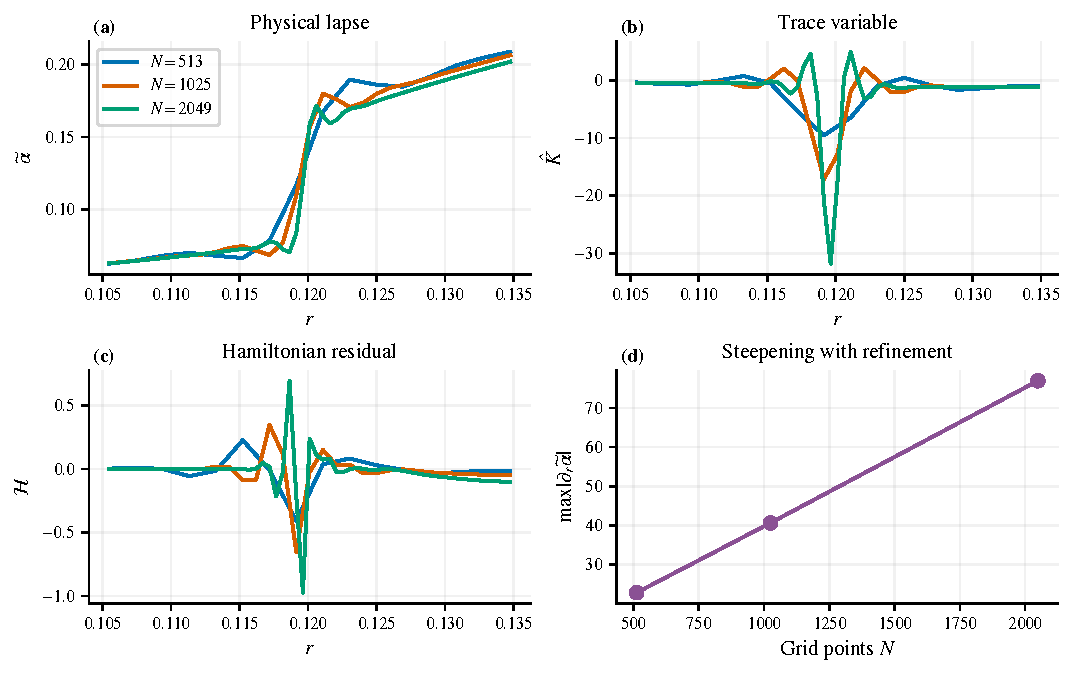
\includegraphics[width=\textwidth]{wormhole_front}
 \caption{Pre-telegrapher baseline: failed $\nu=1$ wormhole trial with the modified logarithmic source, shown at the exact saved time $t=2.5$. The physical lapse steepens, $\Kh$ develops a narrow spike, and the local Hamiltonian error grows under refinement. The gradient diagnostic in (d) uses second-order differentiation of saved profiles; it is not the evolution stencil. This is evidence of unresolved steepening, not a proof of a continuum shock.}
 \label{fig:front}
\end{figure*}

\section{Canceled spherical equations for the metric-freezing sector}
\label{app:equations}
For reproducibility, we give the baseline constant-damping, Appendix-C-style vacuum equations for $g=1$. Let primes denote $\partial_r$, $p=\Kh$, $K=p+2\Th$, $d=K+3$, $c=\chi-1$, $u=\alpha-A$, $v=\beta+r$, and $w=\beta r/\alpha$. For each field $q$, write $q_t=R_q+S_q/\Omega$. All the following expressions retain off-constraint fields. They are algebraic rearrangements of the spherical tensor equations, not numerical background subtraction.

\begin{widetext}
\begin{align}
R_\chi &= \beta c'-2\chi v/r-\alpha\chi\Ar,
\quad S_\chi=\frac{2\chi}{3}(\alpha d-3u-3rv),\label{eq:fullchi}\\
R_{\Ar}&=\beta\Ar'-\frac{2\chi}{3}(u''-u'/r)-\frac23c'\alpha'
 +\frac\alpha3(c''-c'/r)-\frac{\alpha(c')^2}{6\chi}
 +\frac{2\alpha\chi}{3}(\Lambda'-\Lambda/r)+\frac{2\alpha c'\Lambda}{3},
\\ S_{\Ar}&=-\frac{4\alpha r}{3}(c'+\chi\Lambda)+\alpha\Ar(K-w),\label{eq:fullA}\\
R_p&=\beta p'+\frac32\Omega\alpha\Ar^2-\Omega\chi(u''+2u'/r)
 +\frac\Omega2c'\alpha'-3\chi r u'-6Ac+3u-3cu+\frac\alpha2r c',
\\ S_p&=\alpha\left[\frac{d(K-3)}3-3cr^2+\kappa_1(1-\kappa_2)\Th\right],\label{eq:fullp}\\
R_\Th&=\beta\Th'+\alpha rc'+\frac{\Omega\alpha}{2}
 \left[2c''+4c'/r-\frac{5(c')^2}{2\chi}-\frac32\Ar^2+\chi(\Lambda'+2\Lambda/r)\right],
\\ S_\Th&=\alpha\left[\frac{d(K-3)}3-3c-\kappa_1(2+\kappa_2)\Th\right],\label{eq:fullT}\\
R_\Lambda&=\beta\Lambda'+\frac23\Lambda\,\mathrm{div}\beta
 +2\alpha\left[\Ar'+3\Ar/r-\frac{3\Ar c'}{2\chi}\right],
\\ S_\Lambda&=-\alpha(2K/3+\kappa_1)\Lambda-\frac{2\alpha}{3}(2p'+\Th')+4\alpha\Ar r.
\label{eq:fullL}
\end{align}
\end{widetext}
Here $\Lambda=\Lambda^r$, $\mathrm{div}\beta=\beta'+2\beta/r$, and $g_t=0$ follows from the gauge equation. Equation~\eqref{eq:lapse} supplies the lapse, and Eq.~\eqref{eq:W} supplies the shift. Its analytic derivatives are
\begin{align}
 \beta'&=-1+v/r+\tfrac32\alpha\Ar,\\
 \beta''&=\tfrac32(\alpha'\Ar+\alpha\Ar'+\alpha\Ar/r).
\end{align}
The vacuum constraints used in diagnostics are
\begin{align}
 \HH={}&\tfrac23d(K-3)-6c+2\Omega r c'\nonumber\\
 &+\Omega^2\left[2c''+4c'/r-\frac{5(c')^2}{2\chi}-\frac32\Ar^2\right],\\
 \MM={}&\Omega\left(\Ar'+3\Ar/r-\frac{3\Ar c'}{2\chi}\right)
 -\tfrac23K'+2r\Ar.
\end{align}
The remaining Z4 diagnostics are $\Th$ and $Z_r=\Lambda/2$. Regular-center ratios use parity and isotropy limits; the puncture path instead uses its independently derived coefficient equations. Equivalent canceled expressions in $X=\chi/r^2$ and $\ell=(\log X)'$ are used for Eq.~\eqref{eq:trumpet-chart}. Their curvature combination is
\begin{equation}
 2X+2rX\ell+2\chi\ell'-\frac12\chi\ell^2.
\end{equation}
The repository-$\Th$ control subtracts $3\alpha w\Th$ from $S_\Th$. For reference-lapse damping, define $D=-\kappa_1(\alpha-A)$ and add $D(1-\kappa_2)\Th$, $-D(2+\kappa_2)\Th$, and $-D\Lambda$ to $S_p,S_\Th,S_\Lambda$, respectively. The lapse variants were specified in Sec.~\ref{sec:formulation}; none is implicit in Eqs.~\eqref{eq:fullchi}--\eqref{eq:fullL}.

\section{Matter sources and radius-weighted wave equation}
\label{app:matter}
For $\Pi=\bar n(\phi)$ and $g=1$, the additional regular geometric rates are
\begin{align}
 \Delta R_{\Ar}&=-\frac{16\pi}{3}\alpha\chi(\phi')^2,&
 \Delta R_p&=8\pi\alpha\Omega\Pi^2,\\
 \Delta R_\Th&=-4\pi\alpha\Omega[\Pi^2+\chi(\phi')^2],&
 \Delta R_\Lambda&=16\pi\alpha\Pi\phi'.
\end{align}
The constraints receive $\Delta\HH=-8\pi\Omega^2[\Pi^2+\chi(\phi')^2]$ and $\Delta\MM=8\pi\Omega\Pi\phi'$. The scalar variables give
\begin{equation}
 \phi'=\sqrt\chi\left[\Omega f'+\left(-r+\frac{\Omega\chi'}{2\chi}\right)f\right].
\end{equation}
The radius-weighted equation has potential
\begin{equation}
 \mathcal V=\frac{2m}{\Omega^2R^3}-\frac{\mathcal R_\perp}{\Omega^2},
\end{equation}
where $m$ is the Misner--Sharp mass and $\mathcal R_\perp$ is the physical spacetime angular Ricci eigenvalue implied by the evolved geometry. For the candidate off-constraint system,
\begin{align}
 \mathcal R_\perp={}&-\Omega^2\chi\Lambda/r+\Omega^2\chi'\Lambda/3
 -2\Omega r\chi\Lambda/3\nonumber\\
 &+\kappa_1(1+\kappa_2)\Th.
\end{align}
The repository-$\Th$ control adds $2w\Th$, and the reference-lapse damping control changes the corresponding damping product. Retaining these terms avoids substituting an Einstein constraint into the scalar evolution.

Define $U_0=\alpha(K+3)/3-u-rv$ and $\alpha\bar K_R=-1+\alpha\Ar+U_0/\Omega$. The stored wave system is
\begin{align}
 f_t={}&\beta f'+(\beta/r)f+\alpha P,\\
 P_t={}&\beta P'+(\beta/r+\alpha\bar K_R)P
 +\alpha\chi(f''+2f'/r)\nonumber\\
 &+(\alpha\chi'/2+\chi\alpha')f'
 +\left[\frac{\alpha\chi'/2+\chi\alpha'}r-\alpha\mathcal V\right]f.
\end{align}
The scri closure uses $U_0/\Omega=-U_0'$ and $\mathcal V=0$ in the finite-mass compatible phase, monitoring the unfactored residues separately. These limits have assumptions; fixing a clock does not enforce the entire compatibility hierarchy.

The initial Hamiltonian solve uses
\begin{align}
0={}&\Omega w''+(5\Omega'+2\Omega/r)w'-15w
 -\tfrac{15}{2}\Omega^2w^2-\tfrac{15}{2}\Omega^5w^3\nonumber\\
 &-\tfrac{15}{4}\Omega^8w^4-\tfrac34\Omega^{11}w^5
 +\pi(1+\Omega^3w)\frac{(\phi')^2}{\Omega^2}.
\end{align}
Evenness and $w'(1)=-3w(1)$ select the regular branch. For the Gaussian input the outer matter term is below binary64 resolution at the endpoint; the numerical datum there is zero. Residual precision and the subsequent conversion to binary64 are reported separately.

\section{Evidence provenance and reproducibility}
\label{app:repro}
The experiment is isolated on branch \code{codex/hyperboloidal-elliptic-shift-1d}. Its preserved baseline is \code{f5d99045e016}, and the original manuscript used numerical implementation \code{a0c1d6aa3} (compiled API 32). The telegrapher follow-up uses its separately frozen geometry and relaxation libraries; complete inputs and executable/source digests are exported in \code{data/telegraph/}. Older experiments use their own frozen source trees and libraries; a later API number does not retroactively validate them. The manuscript and newest analysis artifacts are separate from that numerical implementation commit.

Each evolution records inputs, command, source hashes, native/compiled library hashes, diagnostics, and checkpoint ancestry. Continuation requires the exact saved source and executable binding. The domain-transfer event is separately recorded and is not a relaxed restart. Paused runs are excluded from completed-result plots. No production branch was merged. The original paused trajectories were not resumed; the telegrapher follow-up consists of separately authorized local runs. At the user-requested finest-grid stopping point, further numerical experiments were stopped and any incomplete controls are labeled explicitly.

The accompanying \code{data/evidence.json} contains the existing review records and selected history columns used here. \code{data/manifests/} retains the plotted runs' complete bindings and inputs. Selected inner profiles are supplied as compressed NumPy arrays. \code{source-manifest.json} maps the original export to repository-relative paths and SHA-256 digests; \code{data/telegraph/source-manifest.json} does the same for the follow-up. The \code{make_figures.py} script regenerates the eight original figures using only this portable bundle; \code{make_telegraph_figures.py} regenerates the five follow-up figures from the exported data. It performs plotting, not evolution. The separate \code{collect_evidence.py} script documents how the bundle was assembled from the original archive. The failure inventory includes explicitly failed/rejected manifests and identifies their paths and hashes; completed-but-unaccepted experiments remain visible in the manuscript.

The principal evidence associations are:
\begin{itemize}
 \item Figs.~\ref{fig:gauge}--\ref{fig:arithmetic}: the compensated finite-pulse trajectory review, local-subtraction trajectory review, and independent arithmetic controls.
 \item Fig.~\ref{fig:endpoint}: the coupled elliptic-mode diagnosis and original pulse trajectory review.
 \item Fig.~\ref{fig:cmc}: the symmetric CMC-source/reference-damping assessment and saved histories.
 \item the pre-telegrapher baseline in Fig.~\ref{fig:front}: exact $t=2.5$ profiles from the $\nu=1$ physical-log wormhole family.
 \item Fig.~\ref{fig:domain}: the completed global-profile retained-domain matrix and same-grid compact-profile control.
 \item Figs.~\ref{fig:tele-lapse}--\ref{fig:tele-rays}: completed three-grid telegrapher trajectories, spatial acceptance review, stage-ray convergence review, and independently reconstructed constraint/horizon histories in \code{data/telegraph/}.
 \item Fig.~\ref{fig:scalar}: the fixed-background scalar oracle, all-stage Bondi dispersal assessment, and failed positive-upwind collapse histories.
 \item Fig.~\ref{fig:tele-long}: the separately authorized $N=1025$ continuation targeting $t=500$, with all saved profiles through $t=43.8$ and the native guard stop at $t=43.8365$. The frozen source and executable bindings, checkpoint ancestry, terminal-status record, and predeclared protocol are retained in \code{data/long-puncture/}.
 \item Fig.~\ref{fig:lapse-stop}: frozen-kernel replay of the unfloored failure and short isolated floor controls in \code{data/lapse-floor/}.
 \item Fig.~\ref{fig:floored-long}: the separate fresh floored trial, including all 1696 saved profiles through $t=84.75$, terminal guard diagnostics, isolated checkpoint replay, and the explicit floor protocol in \code{data/floored-long-puncture/}. The portable \code{make_floored_long_figure.py} script redraws the figure without evolving the system.
\end{itemize}
No statistical error bars are inferred from deterministic resolution sequences. Reference power-law guides in the figures are explicitly labeled; reported self-convergence orders refer to the stated grids, norms, and time windows. The completed telegrapher spatial assessment covers only the stated $t=10$ interval and fixed parameters. The absent independent robustness controls, incomplete physical scenarios, and lack of a demonstrated late-time trumpet limit remain part of the result.

\begin{thebibliography}{99}
\bibitem{VHH2015}
A. Va\~n\'o-Vi\~nuales, S. Husa, and D. Hilditch,
``Spherical symmetry as a test case for unconstrained hyperboloidal evolution,''
Class. Quantum Grav. \textbf{32}, 175010 (2015),
\href{https://arxiv.org/abs/1412.3827v2}{arXiv:1412.3827v2}.
\bibitem{VH2014}
A. Va\~n\'o-Vi\~nuales and S. Husa,
``Unconstrained hyperboloidal evolution of black holes in spherical symmetry with GBSSN and Z4c,''
\href{https://arxiv.org/abs/1412.4801}{arXiv:1412.4801} (2014).
\bibitem{VH2018}
A. Va\~n\'o-Vi\~nuales and S. Husa,
``Spherical symmetry as a test case for unconstrained hyperboloidal evolution II: gauge conditions,''
\href{https://doi.org/10.1088/1361-6382/aaa4e2}{Class. Quantum Grav. (2018)},
\href{https://arxiv.org/abs/1705.06298v3}{arXiv:1705.06298v3}.
\bibitem{VV2023}
A. Va\~n\'o-Vi\~nuales,
``Spherically symmetric black hole spacetimes on hyperboloidal slices,''
Front. Appl. Math. Stat. \textbf{9}, 1206017 (2023),
\href{https://arxiv.org/abs/2304.05384v2}{arXiv:2304.05384v2}.
\bibitem{VV2024}
A. Va\~n\'o-Vi\~nuales,
``Conformal diagrams for stationary and dynamical strong-field hyperboloidal slices,''
Class. Quantum Grav. \textbf{41}, 105003 (2024),
\href{https://arxiv.org/abs/2311.04972v2}{arXiv:2311.04972v2}.
\bibitem{VVValente2024}
A. Va\~n\'o-Vi\~nuales and T. Valente,
``Height-function-based 4D reference metrics for hyperboloidal evolution,''
Gen. Relativ. Gravit. \textbf{56}, 135 (2024),
\href{https://arxiv.org/abs/2408.08952v2}{arXiv:2408.08952v2}.
\bibitem{Alcubierre2005}
M. Alcubierre,
``Are gauge shocks really shocks?,''
Class. Quantum Grav. \textbf{22}, 4071 (2005),
\href{https://arxiv.org/abs/gr-qc/0503030v2}{arXiv:gr-qc/0503030v2}.
\bibitem{BaumgarteHilditch2022}
T. W. Baumgarte and D. Hilditch,
``Shock-avoiding slicing conditions: tests and calibrations,''
Phys. Rev. D \textbf{106}, 044014 (2022),
\href{https://arxiv.org/abs/2207.06376}{arXiv:2207.06376}.
\bibitem{Alvares2026}
J. D. \'Alvares and A. Va\~n\'o-Vi\~nuales,
``Charged Scalar Field at Future Null Infinity via Nonlinear Hyperboloidal Evolution,''
\href{https://arxiv.org/abs/2506.15311v4}{arXiv:2506.15311v4} (2026).
\bibitem{PCHIP}
SciPy developers, ``PchipInterpolator,'' SciPy documentation,
\href{https://docs.scipy.org/doc/scipy/reference/generated/scipy.interpolate.PchipInterpolator.html}{online algorithm documentation}
(accessed 26 October 2026).
\bibitem{RK4Dense}
Hipparchus developers, ``ClassicalRungeKuttaStateInterpolator,'' version 4.0.3 API documentation,
\href{https://hipparchus.org/apidocs-4.0.3/org/hipparchus/ode/nonstiff/interpolators/ClassicalRungeKuttaStateInterpolator.html}{online interpolation formula}
(accessed 26 October 2026).
\end{thebibliography}

\end{document}
